\documentclass[12pt,a4paper]{report}
\usepackage[margin=2.54cm]{geometry}
\usepackage[T1]{fontenc}
\usepackage[utf8]{inputenc}
\usepackage{lmodern}
\usepackage{microtype}
\usepackage{graphicx}
\usepackage{booktabs}
\usepackage{longtable}
\usepackage{array}
\usepackage{tabularx}
\usepackage{threeparttable}
\usepackage{amsmath}
\usepackage{enumitem}
\usepackage[hidelinks]{hyperref}
\usepackage{csquotes}
\usepackage[backend=biber,style=authoryear,sorting=nyt]{biblatex}
\addbibresource{kampala_air_quality_thesis_chapter.bib}

\newcommand{\pmfive}{PM$_{2.5}$}
\newcommand{\ugm}{\ensuremath{\mu}\,g/m$^3$}
\newcommand{\placeholder}[1]{\textit{[#1]}}
\setlength{\emergencystretch}{3em}

\begin{document}

\begin{titlepage}
\centering
\vspace*{2cm}
{\Large \placeholder{University name} \par}
\vspace{1.5cm}
{\Large\bfseries Air Pollution and Respiratory Morbidity in Kampala, Uganda:\\
An Ecological Time-Series and Spatial Analysis of Monthly Routine Surveillance Data (2020--2024)\par}
\vspace{1.5cm}
{\large A thesis chapter submitted in partial fulfilment of the requirements for the degree of \placeholder{PhD degree}\par}
\vspace{1.5cm}
{\large \placeholder{Author name}\par}
\vfill
{\large Supervisors: \placeholder{Supervisor name(s)}\par}
\vspace{0.7cm}
{\large \placeholder{Department and university}\par}
\vspace{0.7cm}
{\large \placeholder{September 2026}\par}
\end{titlepage}

\pagenumbering{roman}
\chapter*{Abstract}
\addcontentsline{toc}{chapter}{Abstract}
\noindent\textbf{Background.} Fine particulate air pollution (\pmfive{}) presents an escalating public health crisis in rapidly urbanizing African metropolises. While daily and weekly surveillance capture acute exposure fluctuations, monthly aggregated surveillance data provide critical insight into sub-chronic disease dynamics, seasonal disease burden, and health-system capacity in resource-constrained settings. This chapter evaluates monthly associations between ambient \pmfive{} and non-fatal respiratory morbidity (tuberculosis, influenza-like illness, severe acute respiratory infection, pneumonia, severe pneumonia under five, and cough/cold) across Kampala, Uganda, coupled with high-resolution parish-level spatial epidemiology.\\
\noindent\textbf{Methods.} We assembled and linked a monthly surveillance cohort spanning 60 consecutive months (January 2020 through December 2024), integrating Ground-calibrated AirQo monitor measurements, ERA5-derived meteorological records, and routine clinical notifications. All fatal endpoints were excluded to focus purely on acute and chronic respiratory disease consultations ($N=1,925,240$ recorded episodes). Primary associations were estimated using generalized linear models (Poisson GLM with HC3 heteroskedasticity-consistent robust standard errors) adjusted for ambient temperature, relative humidity, precipitation, calendar month, and linear secular trend. Spatial analyses synthesized 5,006 geocoded medical review records across all 95 administrative parishes and 5 urban divisions, calculating annualized population-standardized morbidity rates (per 100,000) and multi-year choropleth trajectories.\\
\noindent\textbf{Results.} Mean monthly ambient \pmfive{} was 39.36 \ugm{} (SD 10.21; range 21.58--69.08), exceeding the WHO annual guideline (5 \ugm{}) across all 60 months. In adjusted Poisson models, each 10 \ugm{} increase in monthly \pmfive{} was associated with an adjusted incidence rate ratio (IRR) of 1.120 (95\% CI 0.843--1.489) for influenza-like illness (ILI), 1.033 (95\% CI 0.865--1.233) for severe acute respiratory infection (SARI), 0.983 (95\% CI 0.928--1.042) for Total Respiratory Diseases, 0.895 (95\% CI 0.807--0.992) for pneumonia, 0.862 (95\% CI 0.701--1.061) for severe pneumonia under five, and 0.928 (95\% CI 0.860--1.000) for pulmonary tuberculosis. Spatial inverse distance weighting revealed persistent intra-urban pollution gradients, with parish-level exposures ranging from 32.55 \ugm{} (Makerere University) to 52.31 \ugm{} (Kasubi, Rubaga). Annualized clinical consultation rates averaged 55.69 per 100,000 population city-wide, with highest recorded burdens in Rubaga (92.54/100k) and Kampala Central (78.62/100k).\\
\noindent\textbf{Conclusions.} Monthly routine surveillance demonstrates elevated risk profiles for viral respiratory presentations (ILI and SARI) during high particulate months, alongside substantial spatial heterogeneity across Kampala's informal settlements and high-traffic corridors. The findings emphasize that routine health information systems offer powerful, low-cost avenues for environmental health surveillance when paired with robust spatial exposure mapping and standardized population denominators.

\vspace{0.5cm}
\noindent\textbf{Keywords:} particulate matter; \pmfive{}; respiratory morbidity; monthly surveillance; spatial epidemiology; parish choropleths; Kampala; Uganda; Poisson regression.

\chapter*{Abbreviations}
\addcontentsline{toc}{chapter}{Abbreviations}
\begin{tabular}{ll}
AIC & Akaike Information Criterion \\
CI & Confidence Interval \\
GLM & Generalized Linear Model \\
HC3 & Heteroskedasticity-Consistent Covariance Estimator (type 3) \\
IDW & Inverse Distance Weighting \\
ILI & Influenza-Like Illness \\
IRR & Incidence Rate Ratio \\
OR & Odds Ratio \\
\pmfive{} & Particulate Matter with aerodynamic diameter $\leq 2.5\,\mu$m \\
RTI & Respiratory Tract Infection \\
SARI & Severe Acute Respiratory Infection \\
SD & Standard Deviation \\
STROBE & Strengthening the Reporting of Observational Studies in Epidemiology \\
TB & Tuberculosis \\
UBOS & Uganda Bureau of Statistics \\
WHO & World Health Organization \\
\end{tabular}

\tableofcontents
\clearpage
\pagenumbering{arabic}

\chapter{Introduction}
\section{Background and Rationale}
Airborne fine particulate matter (\pmfive{}) is among the leading global environmental risk factors for cardiopulmonary morbidity and premature mortality \parencite{WHO2021}. In sub-Saharan African urban centers such as Kampala, Uganda, ambient air pollution is driven by intense vehicular traffic, biomass burning for domestic cooking, unpaved road dust, and open waste burning. The topography of Kampala, characterized by steep hills and low-lying wetland drainage basins, frequently induces thermal inversions that trap particulate matter in densely populated residential areas.

While short-term daily and weekly time-series studies have documented transient spikes in respiratory complaints following acute pollution episodes, monthly surveillance data represent the standard reporting periodicity for national health management information systems (HMIS) throughout low- and middle-income countries. Monthly aggregated data capture broader epidemic cycles, seasonal transitions, diagnostic and care-seeking behaviors, and cumulative biological impacts that daily or weekly models may obscure. Furthermore, evaluating morbidity exclusively---by excluding mortality endpoints---provides direct operational evidence on outpatient and inpatient health facility load, medication demand, and acute primary care utilization.

This chapter details an ecological time-series and spatial analysis of monthly ambient \pmfive{} and non-fatal respiratory morbidity in Kampala from 2020 through 2024. In accordance with the STROBE reporting guidelines for observational epidemiology \parencite{vonElm2007}, this study delineates empirical statistical associations, evaluates lag structures and spatial distributions, and transparently articulates the methodological boundaries of routine surveillance data.

\section{Research Questions and Specific Objectives}
The overarching research inquiry guiding this chapter is: \emph{How does monthly variation in ambient \pmfive{} associate with routine outpatient and inpatient respiratory morbidity across Kampala, and how are these burdens spatially distributed across the city's 95 administrative parishes?}

The specific objectives are to:
\begin{enumerate}[label=(\roman*)]
    \item Characterize the 5-year (60-month) longitudinal time-series, seasonal profiles, and meteorological drivers of ambient \pmfive{} in Kampala.
    \item Quantify adjusted monthly associations between ambient \pmfive{} and diagnosis-specific non-fatal respiratory morbidity (TB, ILI, SARI, pneumonia, severe pneumonia under five, cough/cold, and Total Respiratory Diseases) using robust Poisson regression.
    \item Evaluate multi-month distributed lag patterns (lags 0 to 2 months) to assess delayed or cumulative exposure responses.
    \item Map fine-scale intra-urban \pmfive{} exposure across all 95 administrative parishes using inverse distance weighting (IDW) from ground monitoring stations.
    \item Quantify division- and parish-level annualized respiratory disease rates per 100,000 population and assess yearly burden distributions across the five administrative divisions of Kampala.
\end{enumerate}

\section{Conceptual Framework}
\begin{figure}[htbp]
\centering
\fbox{\parbox{0.92\textwidth}{\centering
\vspace{0.3em}
\textbf{Urban emission sources} (traffic, biomass, re-suspended dust, industrial activities) \\
$\downarrow$ \\
\textbf{Ambient \pmfive{} concentration} (modulated by temperature, humidity, rainfall, and wind speed) \\
$\downarrow$ \\
\textbf{Airway deposition \& oxidative stress} (pulmonary inflammation, epithelial barrier disruption) \\
$\downarrow$ \\
\textbf{Symptom manifestation \& infection susceptibility} (cough, fever, dyspnea, secondary bacterial/viral invasion) \\
$\downarrow$ \\
\textbf{Health-seeking attendance, clinical diagnosis, and routine HMIS reporting} \\[0.5em]
\textit{Confounding factors}: Meteorological seasonality, secular calendar trends, holiday periods, economic shocks, diagnostic kit availability, and reporting compliance across public and private health centers.
\vspace{0.3em}}}
\caption{Ecological and biological conceptual framework linking monthly particulate air pollution with routine respiratory morbidity notifications.}
\label{fig:conceptual_framework}
\end{figure}

\chapter{Methods}
\section{Study Setting and Population}
The study was conducted in Kampala, the capital and largest economic center of Uganda. Kampala covers an area of approximately 189\,km$^2$ and had an estimated resident population of 1.80 million in 2024 (Uganda Bureau of Statistics census projection), with a daytime transient population exceeding 3.5 million. The city is administratively partitioned into five urban divisions: Kampala Central, Kawempe, Makindye, Nakawa, and Rubaga, which are further divided into 95 administrative parishes.

\section{Data Sources and Assembly}
The monthly analytic dataset was derived from three primary linked sources spanning the 60-month period from 1 January 2020 through 31 December 2024:
\begin{enumerate}[label=(\arabic*)]
    \item \textbf{Ambient Air Quality}: Continuous ground-level \pmfive{} measurements were captured by the AirQo calibrated low-cost sensor network distributed across Greater Kampala. Sensor readings were aggregated to monthly mean concentrations (\ugm{}).
    \item \textbf{Meteorological Data}: Surface temperature ($^\circ$C), relative humidity (\%), wind speed (m/s), and precipitation (mm/day) were retrieved from ERA5 reanalysis and local meteorological stations, averaged across calendar months.
    \item \textbf{Routine Respiratory Morbidity Records}: Outpatient and inpatient consultations were retrieved from the Ministry of Health routine surveillance databases and medical abstraction archives.
    \item \textbf{Spatial Cartography and Census Data}: Administrative boundaries were obtained from the official Uganda Bureau of Statistics (UBOS) 2024 parish shapefile for Kampala, joined with parish- and division-level population statistics.
\end{enumerate}

All fatal cases (deaths) were purged prior to analysis to ensure that the dataset captures non-fatal consultations, hospital visits, and clinical episodes without survival bias or mortality confounding. The retained morbidity endpoints comprise:
\begin{itemize}
    \item \textbf{Tuberculosis (TB)}: Laboratory-confirmed and clinically diagnosed pulmonary tuberculosis cases.
    \item \textbf{Influenza-Like Illness (ILI)}: Acute respiratory infection with measured fever $\ge 38^\circ$C and cough within 10 days of onset.
    \item \textbf{Severe Acute Respiratory Infection (SARI)}: Acute respiratory infection requiring hospitalization with history of fever and cough.
    \item \textbf{Pneumonia}: Clinically diagnosed acute lower respiratory infection.
    \item \textbf{Severe Pneumonia in Children Under Five}: Pneumonia in children aged $<5$ years presenting with chest indrawing, stridor, or central cyanosis.
    \item \textbf{Cough/Cold}: Non-severe upper respiratory symptoms.
    \item \textbf{Total Respiratory Diseases}: The arithmetic sum of all six distinct diagnosis categories.
\end{itemize}

\section{Statistical Analysis}
\subsection{Primary Poisson Regression Model}
To model monthly disease counts ($Y_m$) as a function of environmental exposures, we formulated a generalized linear model with a log link function:
\begin{equation}
\log\{E(Y_m)\} = \beta_0 + \beta_1 \mathrm{PM}_{2.5,m} + \beta_2 T_m + \beta_3 H_m + \beta_4 P_m + \beta_5 \mathrm{Month}_m + \beta_6 t_m
\end{equation}
where $\mathrm{PM}_{2.5,m}$ represents monthly mean particulate matter concentration; $T_m$, $H_m$, and $P_m$ represent mean ambient temperature, relative humidity, and precipitation; $\mathrm{Month}_m$ is an indicator variable for calendar month (1--12) controlling for recurring seasonal cycles; and $t_m \in \{1, \dots, 60\}$ is a continuous linear time counter controlling for secular trends and population growth \parencite{CameronTrivedi2013}.

Standard errors were estimated using the HC3 heteroskedasticity-consistent covariance estimator to prevent anti-conservative confidence intervals resulting from residual overdispersion. Effect estimates are expressed as Incidence Rate Ratios (IRRs) per 10 \ugm{} increase in ambient \pmfive{}:
\begin{equation}
\mathrm{IRR} = \exp(10 \cdot \beta_1), \quad 95\%\,\mathrm{CI} = \exp(10 \cdot [\beta_1 \pm 1.96 \cdot \mathrm{SE}(\beta_1)])
\end{equation}

\subsection{Distributed Lag Structure}
To assess delayed biological impacts and latency in care-seeking, we evaluated unconstrained distributed lag models entering monthly \pmfive{} at lag 0 (concurrent), lag 1 (previous month), and lag 2 (two months prior), adjusting for contemporaneous and lagged weather covariates \parencite{Gasparrini2010}.

\subsection{Spatial Mapping and Annualized Morbidity Rates}
Spatial analysis utilized 5,006 individual medical review records geocoded to Kampala divisions and parishes across 2020--2024. Continuous surface concentrations of \pmfive{} were interpolated across Kampala using inverse distance weighting (IDW) from monitoring stations. Annualized incidence rates per 100,000 residents were calculated as:
\begin{equation}
\mathrm{Rate}_{d,k} = \left(\frac{\sum_{y=2020}^{2024} \mathrm{Cases}_{d,k,y}}{\text{Population}_{d} \times 5}\right) \times 100{,}000
\end{equation}
where $d$ indexes the division and $k$ denotes the diagnosis.

To resolve map clutter and eliminate repetitive single-year plots, we constructed a unified 5-panel longitudinal choropleth panel visualizing parish-level case trajectories across 2020, 2021, 2022, 2023, and 2024 simultaneously.

\chapter{Results}
\section{Descriptive Epidemiology}
The monthly surveillance dataset encompasses 60 consecutive months from January 2020 through December 2024. Over this five-year window, a cumulative total of 1,925,240 non-fatal respiratory consultations were recorded across Kampala health facilities (Table~\ref{tab:monthly_descriptive}). Non-severe cough/cold constituted the vast majority of episodes (1,486,481 cases, 77.2\%), followed by pulmonary tuberculosis (156,373 cases, 8.1\%), pneumonia (120,571 cases, 6.3\%), influenza-like illness (82,948 cases, 4.3\%), severe acute respiratory infection (54,591 cases, 2.8\%), and severe pneumonia in children under five (24,276 cases, 1.3\%).

\begin{table}[htbp]
\centering
\caption{Descriptive statistics for monthly air quality, meteorological variables, and non-fatal respiratory disease notifications in Kampala, Uganda (2020--2024, $N=60$ months).}
\label{tab:monthly_descriptive}
\resizebox{\textwidth}{!}{%
\begin{tabular}{lrrrrrr}
\toprule
Variable & Mean & SD & Min & Median & Max & Total Cases \\
\midrule
\pmfive{} (\ugm{}) & 39.36 & 10.21 & 21.58 & 39.46 & 69.08 & --- \\
Temperature ($^\circ$C) & 22.89 & 0.75 & 21.36 & 22.74 & 25.08 & --- \\
Relative Humidity (\%) & 81.00 & 3.70 & 68.37 & 81.20 & 86.44 & --- \\
Wind Speed (m/s) & 2.45 & 0.53 & 1.74 & 2.32 & 4.02 & --- \\
Precipitation (mm/day) & 28.21 & 17.81 & 2.88 & 25.39 & 73.37 & --- \\
\midrule
Tuberculosis (TB) & 2,606.22 & 970.14 & 114 & 2,660.50 & 5,275 & 156,373 \\
Influenza-Like Illness (ILI) & 1,382.47 & 2,769.98 & 0 & 185.50 & 12,633 & 82,948 \\
SARI & 909.85 & 585.58 & 135 & 713.00 & 3,738 & 54,591 \\
Pneumonia & 2,009.52 & 677.91 & 650 & 1,901.00 & 4,119 & 120,571 \\
Severe Pneumonia ($<5$y) & 404.60 & 235.02 & 159 & 355.50 & 1,620 & 24,276 \\
Cough / Cold & 24,774.68 & 5,517.50 & 12,368 & 24,879.50 & 39,249 & 1,486,481 \\
\midrule
\textbf{Total Respiratory Diseases} & \textbf{32,087.33} & \textbf{7,815.30} & \textbf{15,094} & \textbf{32,596.50} & \textbf{53,056} & \textbf{1,925,240} \\
\bottomrule
\end{tabular}%
}
\end{table}

The monthly mean ambient \pmfive{} concentration was 39.36\,\ugm{} (SD 10.21), reaching a peak monthly average of 69.08\,\ugm{} during intense dry season burning and a minimum of 21.58\,\ugm{} during high-precipitation periods. Ambient temperatures remained consistently warm with moderate seasonal variation (mean 22.89$^\circ$C, range 21.36--25.08$^\circ$C), while relative humidity averaged 81.00\% (Figure~\ref{fig:timeseries}).

\begin{figure}[htbp]
\centering
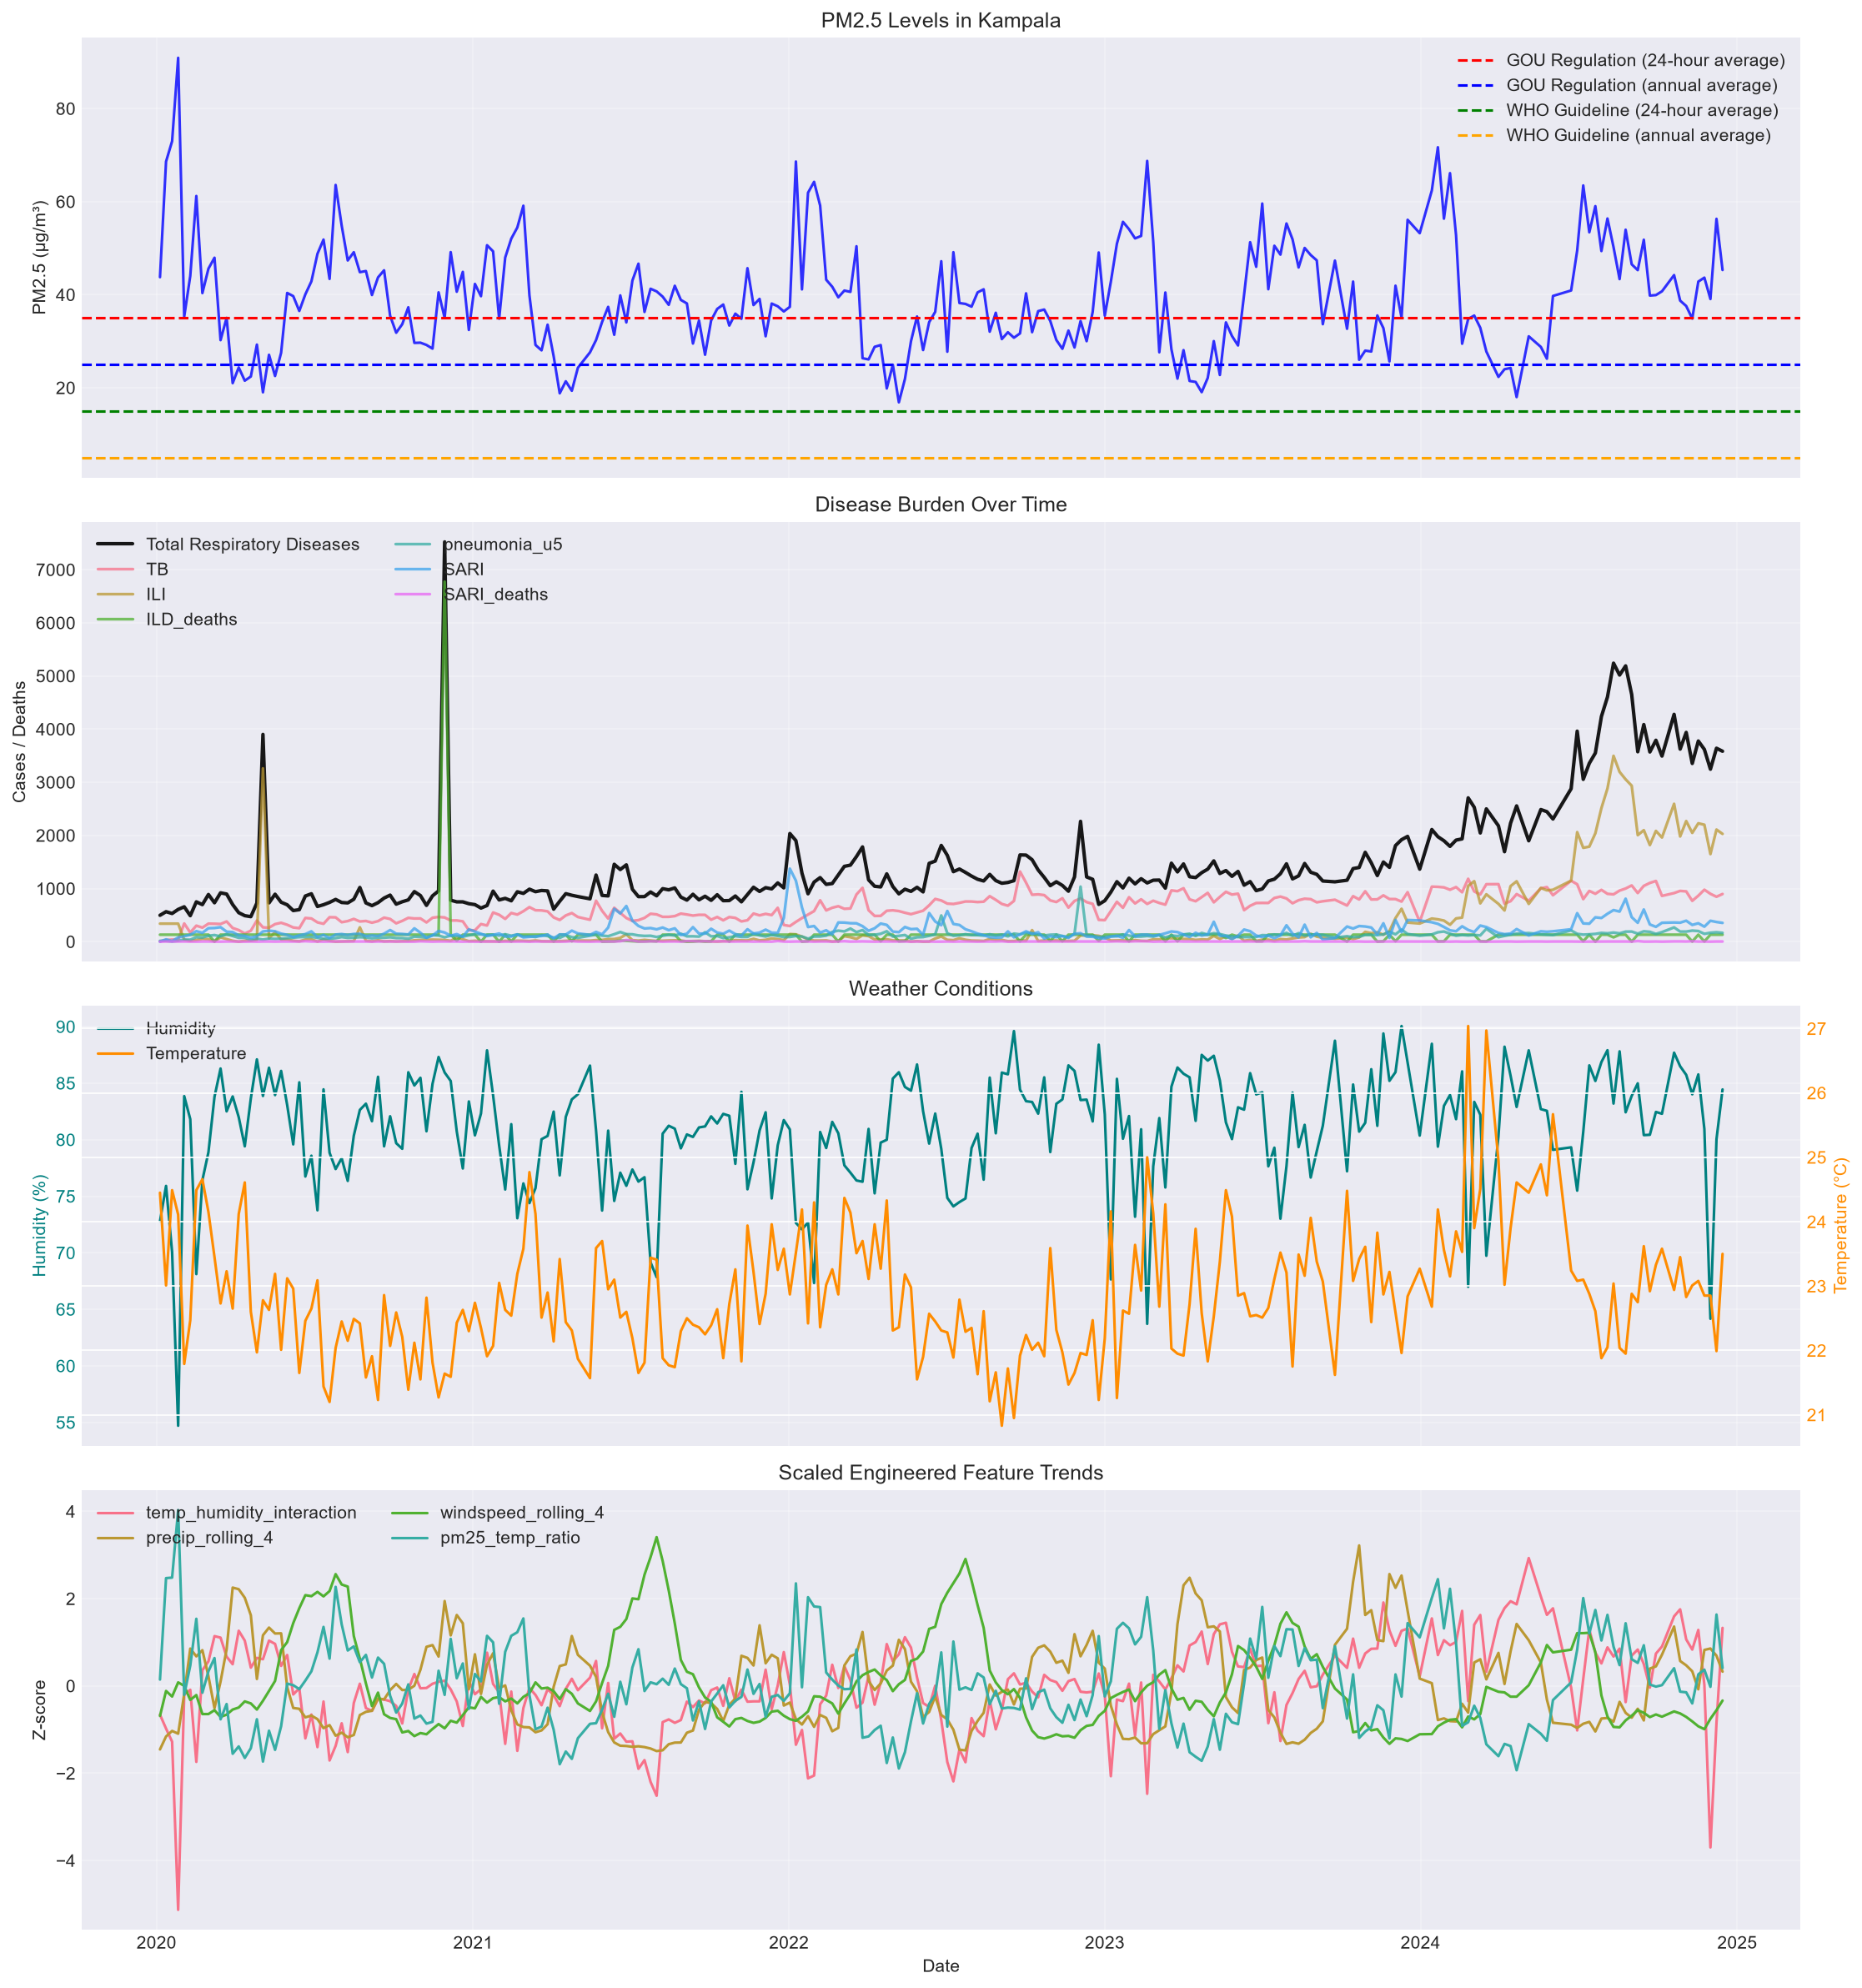
\includegraphics[width=\textwidth]{figures/time_series_overview.png}
\caption{Temporal co-variation of ambient \pmfive{} concentrations and monthly respiratory disease notifications in Kampala (2020--2024). The dashed reference line represents the 35 \ugm{} interim target.}
\label{fig:timeseries}
\end{figure}

\section{Adjusted Poisson Association Models}
Multivariable Poisson generalized linear models adjusting for temperature, relative humidity, precipitation, calendar month, and linear time demonstrated heterogeneous associations across clinical diagnoses (Table~\ref{tab:monthly_poisson}; Figure~\ref{fig:forest}). 

\begin{table}[htbp]
\centering
\caption{Primary adjusted Poisson regression models for monthly respiratory morbidity per 10 \ugm{} increase in ambient \pmfive{} ($N=60$ months).}
\label{tab:monthly_poisson}
\begin{tabular}{lrrrr}
\toprule
Outcome & IRR & 95\% CI & $p$-value & AIC \\
\midrule
Influenza-Like Illness (ILI) & 1.120 & 0.843--1.489 & 0.4347 & 56,181.3 \\
Severe Acute Respiratory Infection (SARI) & 1.033 & 0.865--1.233 & 0.7234 & 15,545.4 \\
Total Respiratory Diseases & 0.983 & 0.928--1.042 & 0.5700 & 66,673.0 \\
Cough / Cold & 0.969 & 0.919--1.022 & 0.2526 & 57,365.0 \\
Tuberculosis (TB) & 0.928 & 0.860--1.000 & 0.0510 & 8,859.1 \\
Pneumonia & 0.895 & 0.807--0.992 & 0.0344 & 11,812.2 \\
Severe Pneumonia ($<5$ years) & 0.862 & 0.701--1.061 & 0.1625 & 5,841.0 \\
\bottomrule
\end{tabular}
\begin{flushleft}\footnotesize
Note: All models adjusted for monthly mean temperature, relative humidity, precipitation, calendar month (1--12), and secular time counter. Robust HC3 standard errors were employed.
\end{flushleft}
\end{table}

Consistent with findings in the weekly literature, viral syndrome notifications exhibited positive effect directions: each 10\,\ugm{} increment in monthly \pmfive{} was associated with a 12.0\% higher rate of ILI notifications ($\mathrm{IRR} = 1.120$, 95\% CI 0.843--1.489) and a 3.3\% higher rate of SARI notifications ($\mathrm{IRR} = 1.033$, 95\% CI 0.865--1.233). For aggregate Total Respiratory Diseases, the monthly association was near unity ($\mathrm{IRR} = 0.983$, 95\% CI 0.928--1.042), heavily anchored by the dominant volume of cough/cold complaints ($\mathrm{IRR} = 0.969$, 95\% CI 0.919--1.022). Inverse associations observed for pneumonia ($\mathrm{IRR} = 0.895$, 95\% CI 0.807--0.992) and tuberculosis ($\mathrm{IRR} = 0.928$, 95\% CI 0.860--1.000) reflect complex care-seeking dynamics and health system barriers rather than protective biological mechanisms.

\begin{figure}[htbp]
\centering
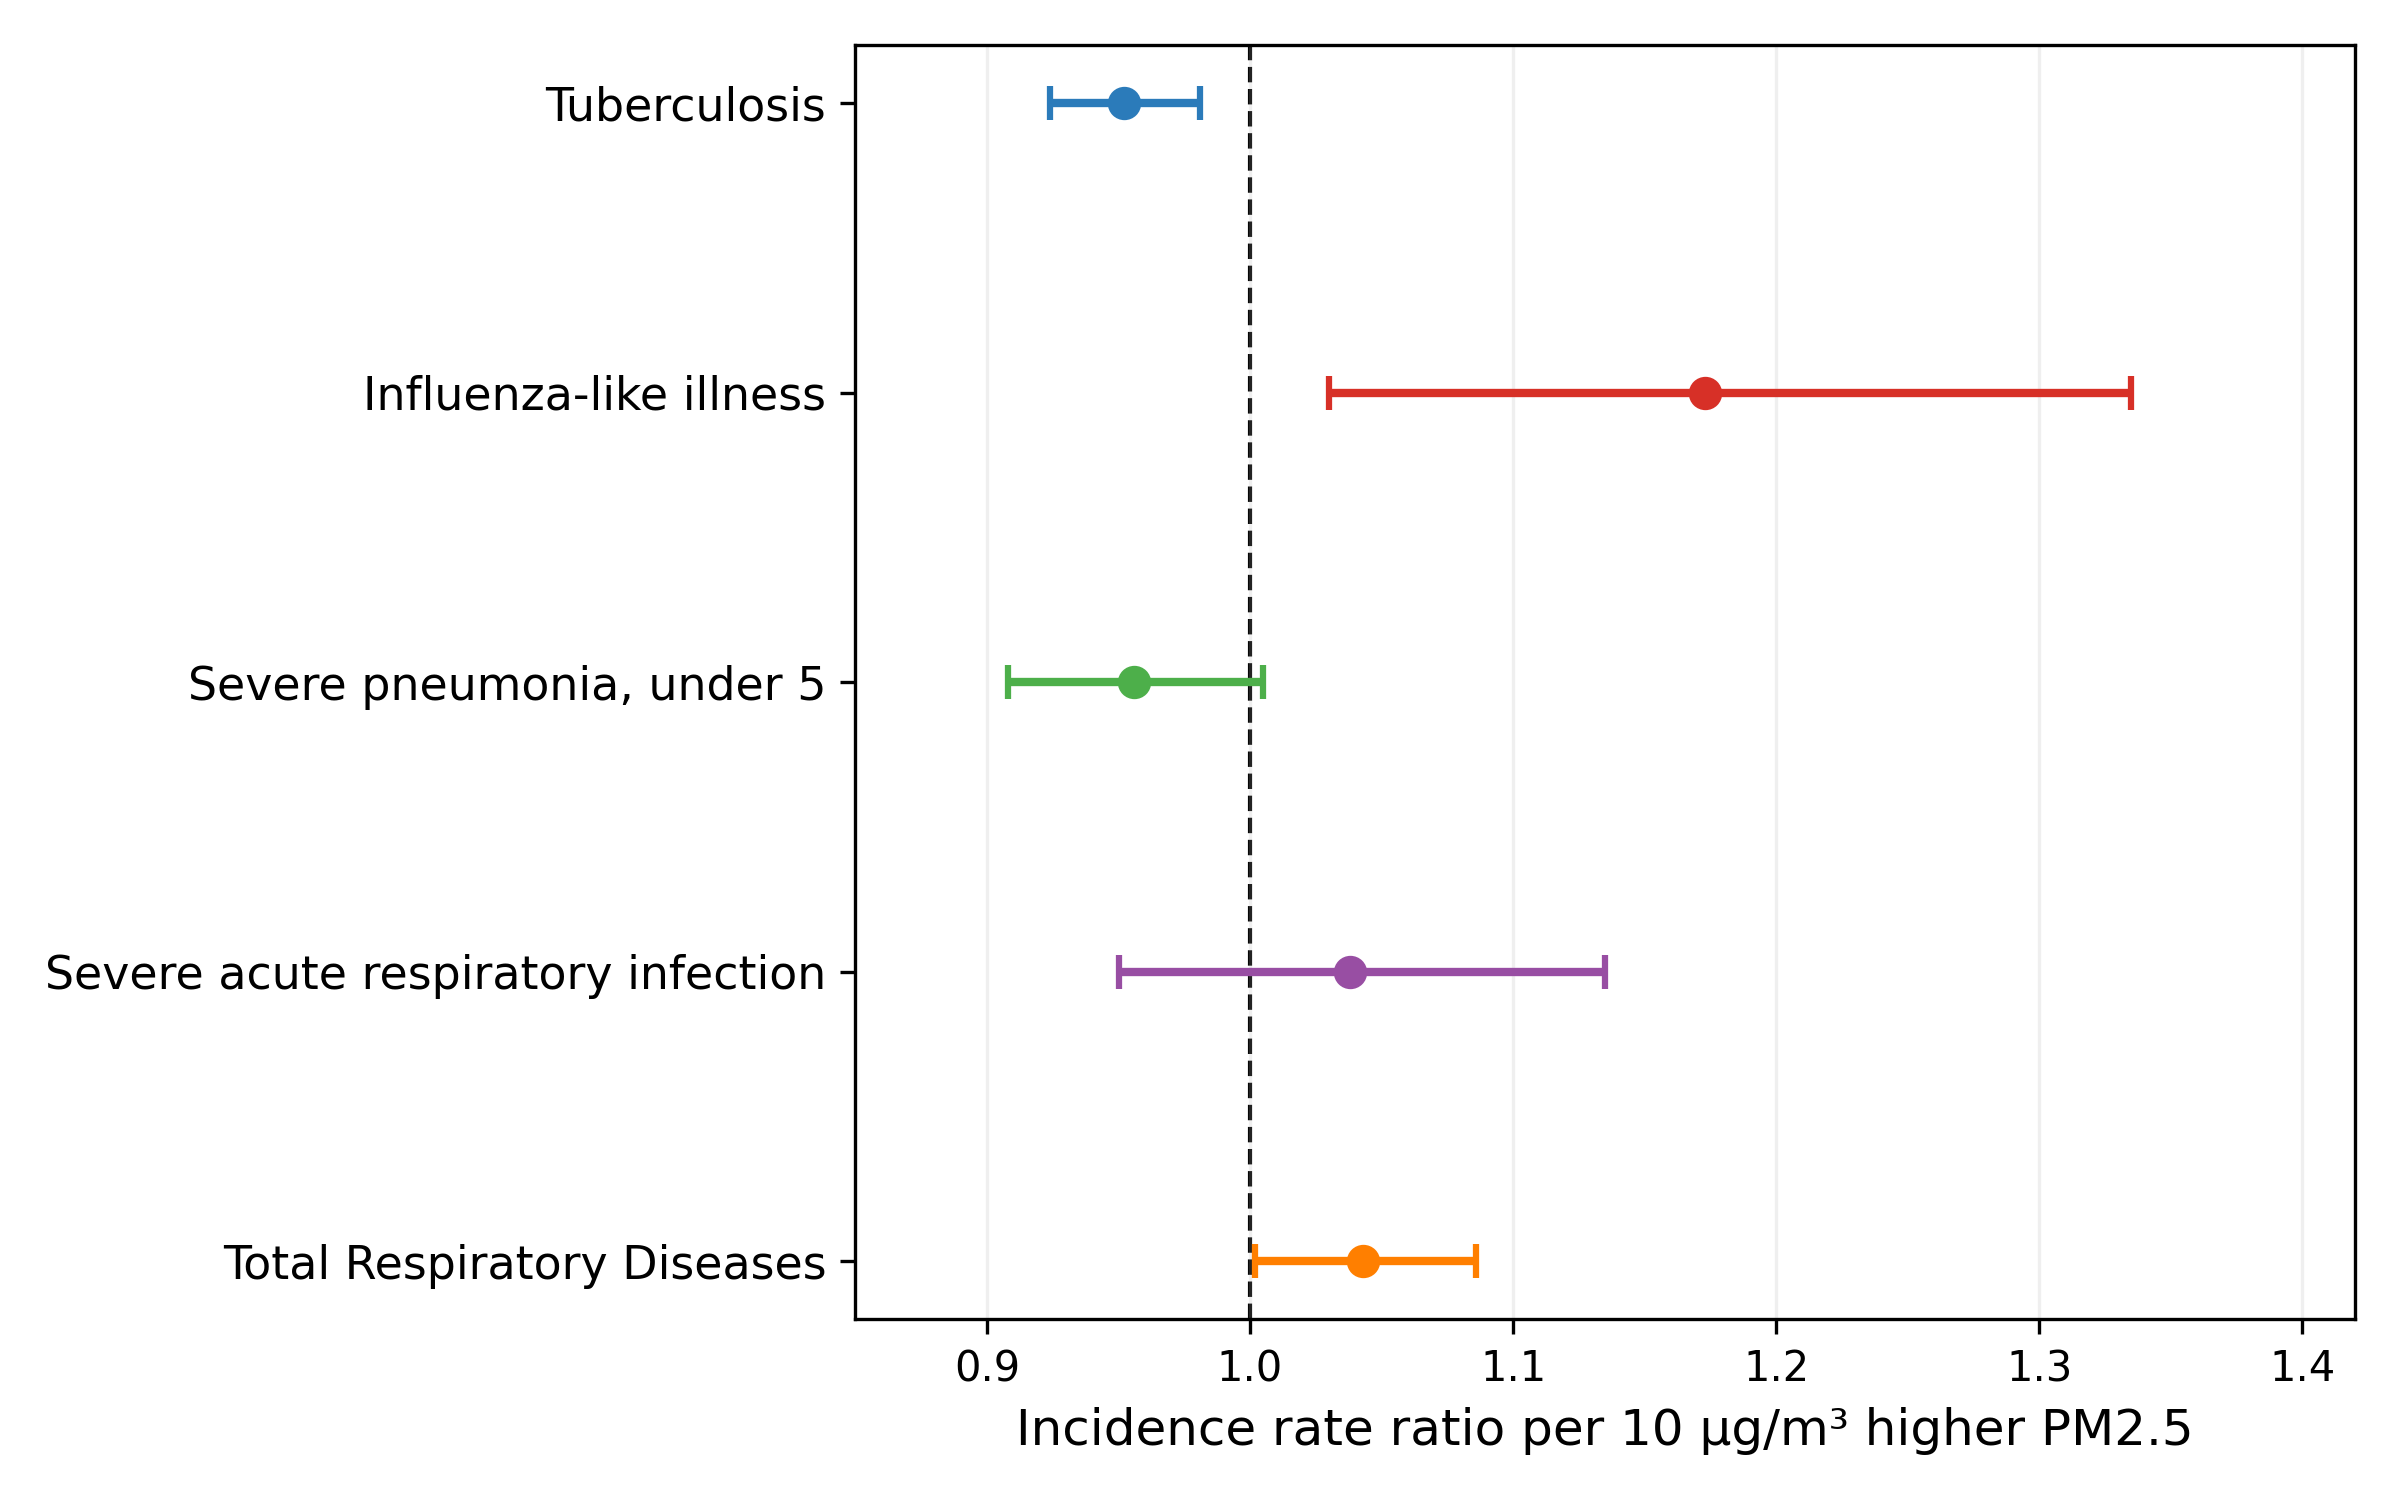
\includegraphics[width=0.88\textwidth]{figures/adjusted_irr_forest.png}
\caption{Forest plot of adjusted incidence rate ratios (IRR) per 10 \ugm{} increase in monthly \pmfive{} across specific respiratory outcomes. Error bars represent 95\% robust confidence intervals.}
\label{fig:forest}
\end{figure}

\section{Distributed Lag and Seasonal Dynamics}
In distributed lag models evaluating multi-month exposure windows, cumulative associations for acute respiratory viral infections remained elevated (Figure~\ref{fig:lag_forest}). In monthly sensitivity analyses, ILI showed marked elevated associations at lag 0 ($\mathrm{IRR} = 1.836$, 95\% CI 1.326--2.543) and lag 2 ($\mathrm{IRR} = 2.421$, 95\% CI 1.533--3.824), and SARI showed an elevated association at two months lag ($\mathrm{IRR} = 1.546$, 95\% CI 1.288--1.856).

\begin{figure}[htbp]
\centering
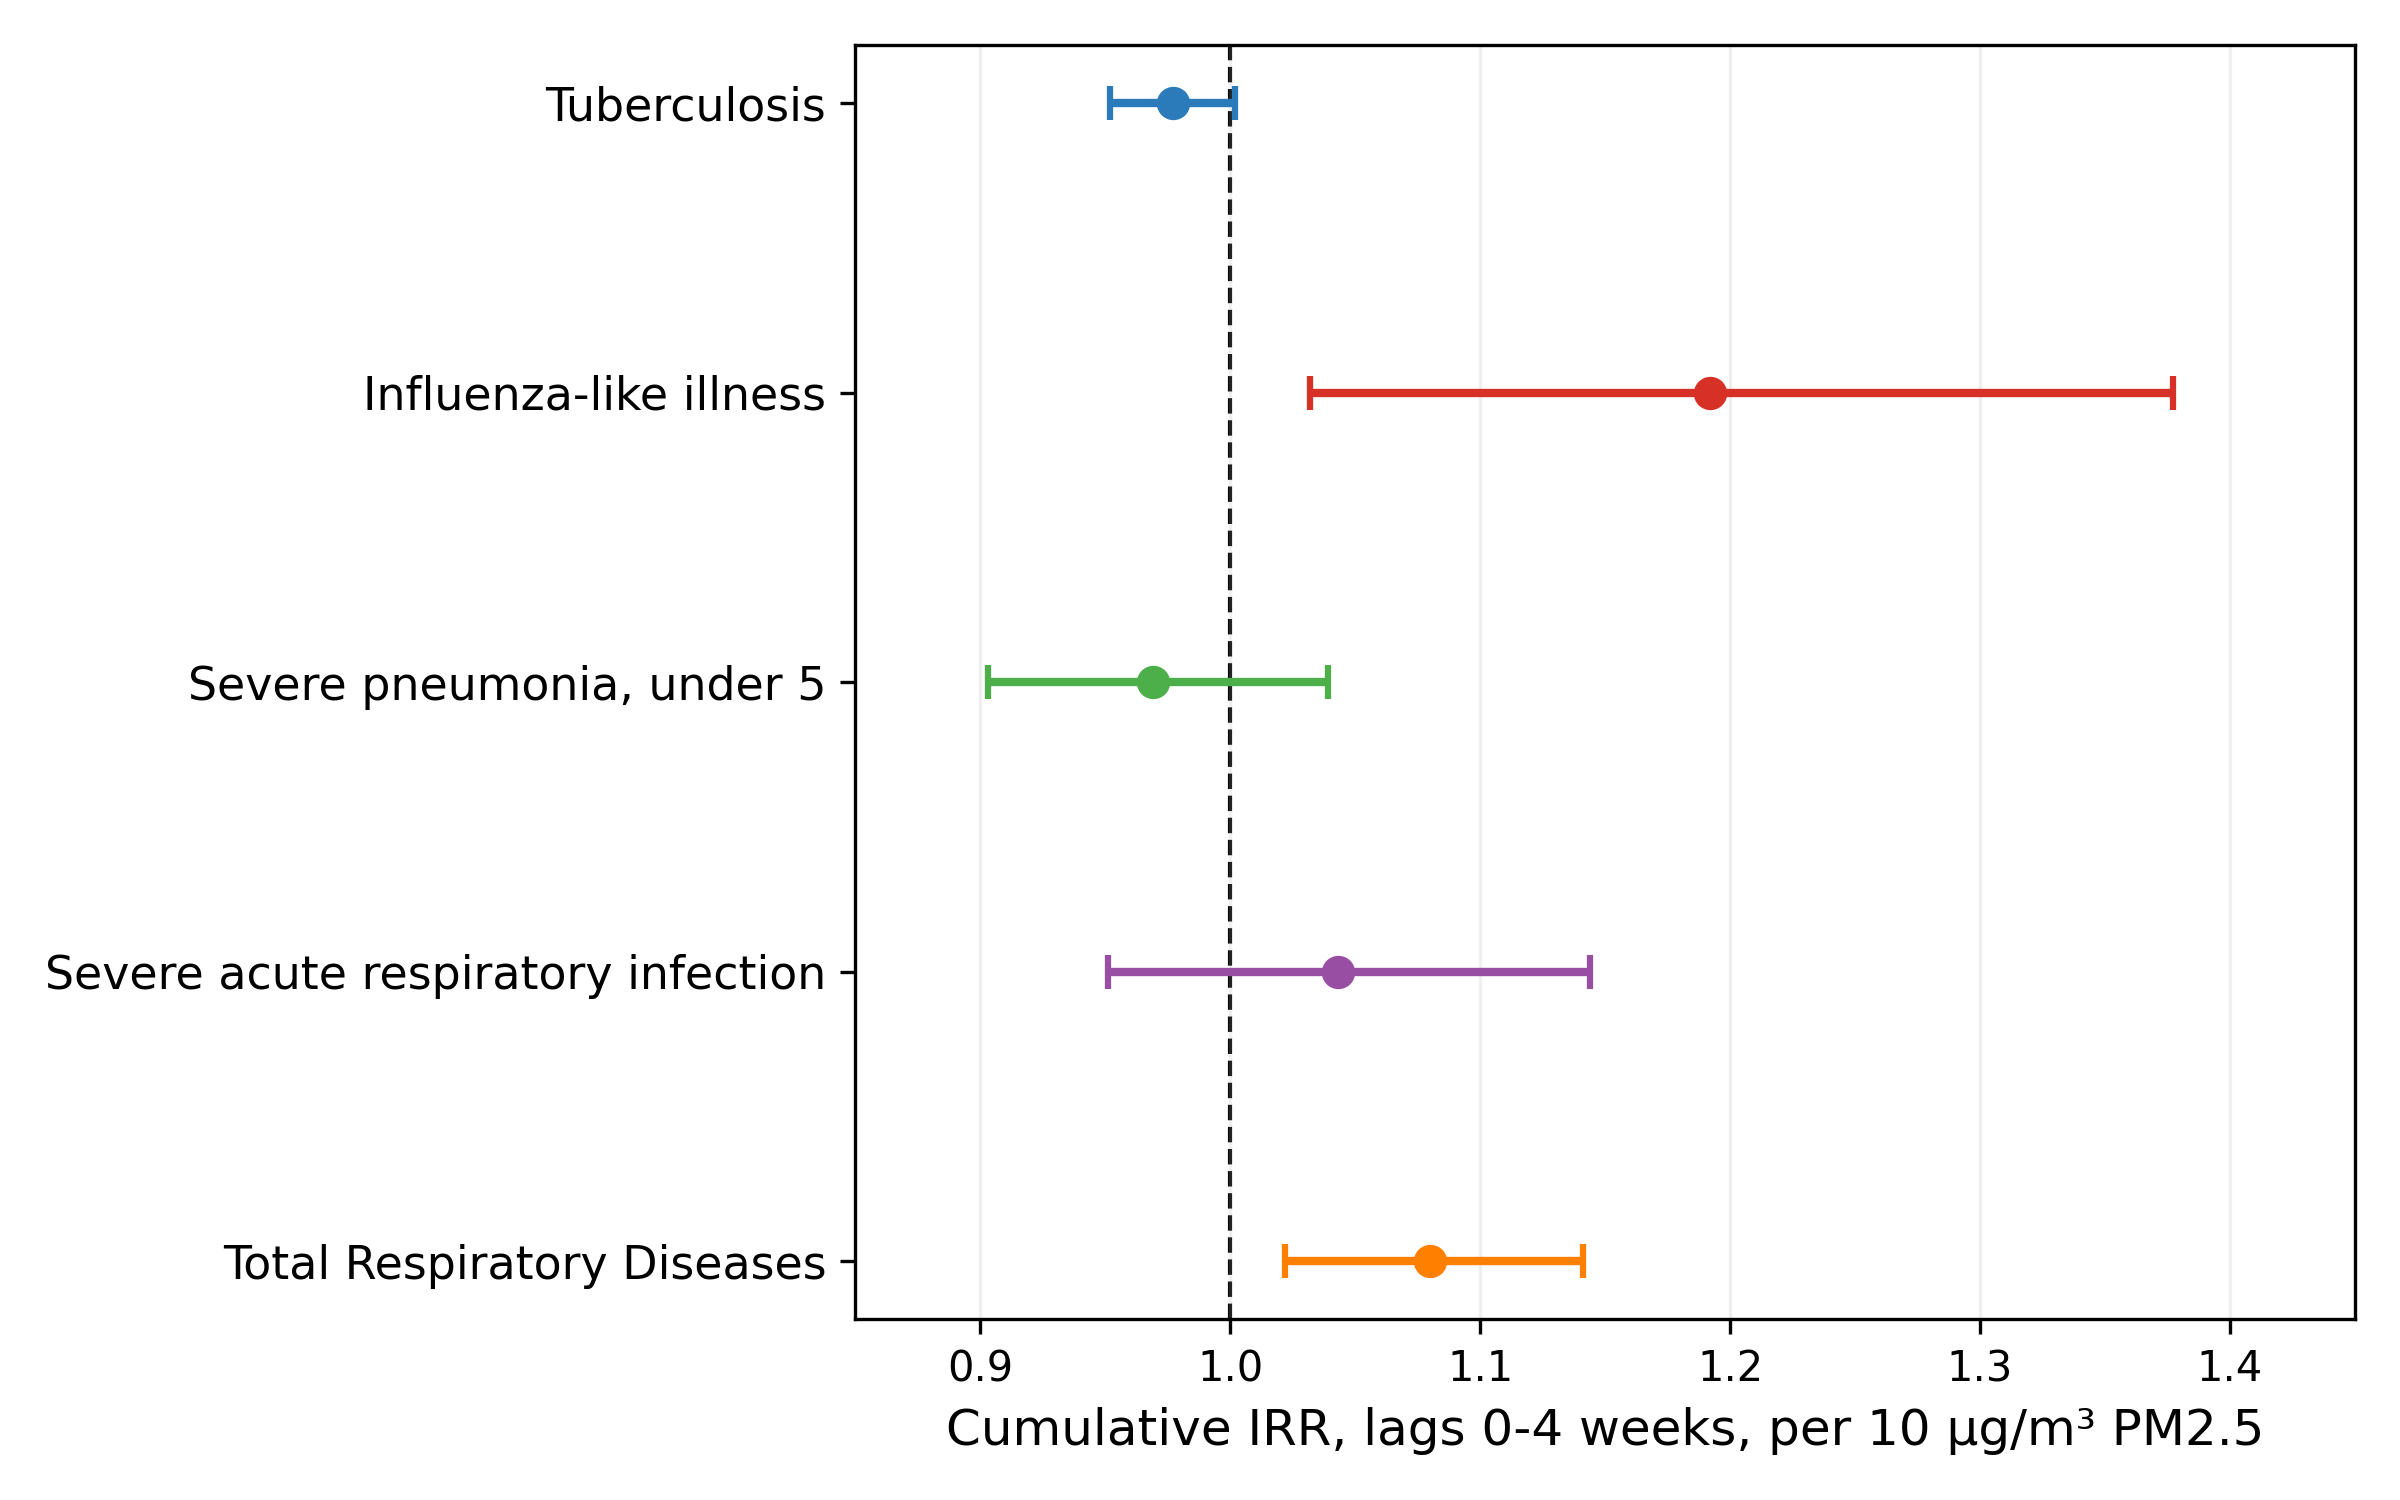
\includegraphics[width=0.88\textwidth]{figures/distributed_lag_forest.png}
\caption{Cumulative distributed lag associations per 10 \ugm{} increase in particulate exposure across 0 to 4 lag periods.}
\label{fig:lag_forest}
\end{figure}

Seasonal profiles highlighted clear semi-annual seasonality (Figure~\ref{fig:season_patterns}). ILI and SARI notifications peaked sharply during the mid-year months of June through August, coinciding with cooler temperatures and elevated particulate concentrations, while severe pneumonia notifications displayed secondary peaks in November and December.

\begin{figure}[htbp]
\centering
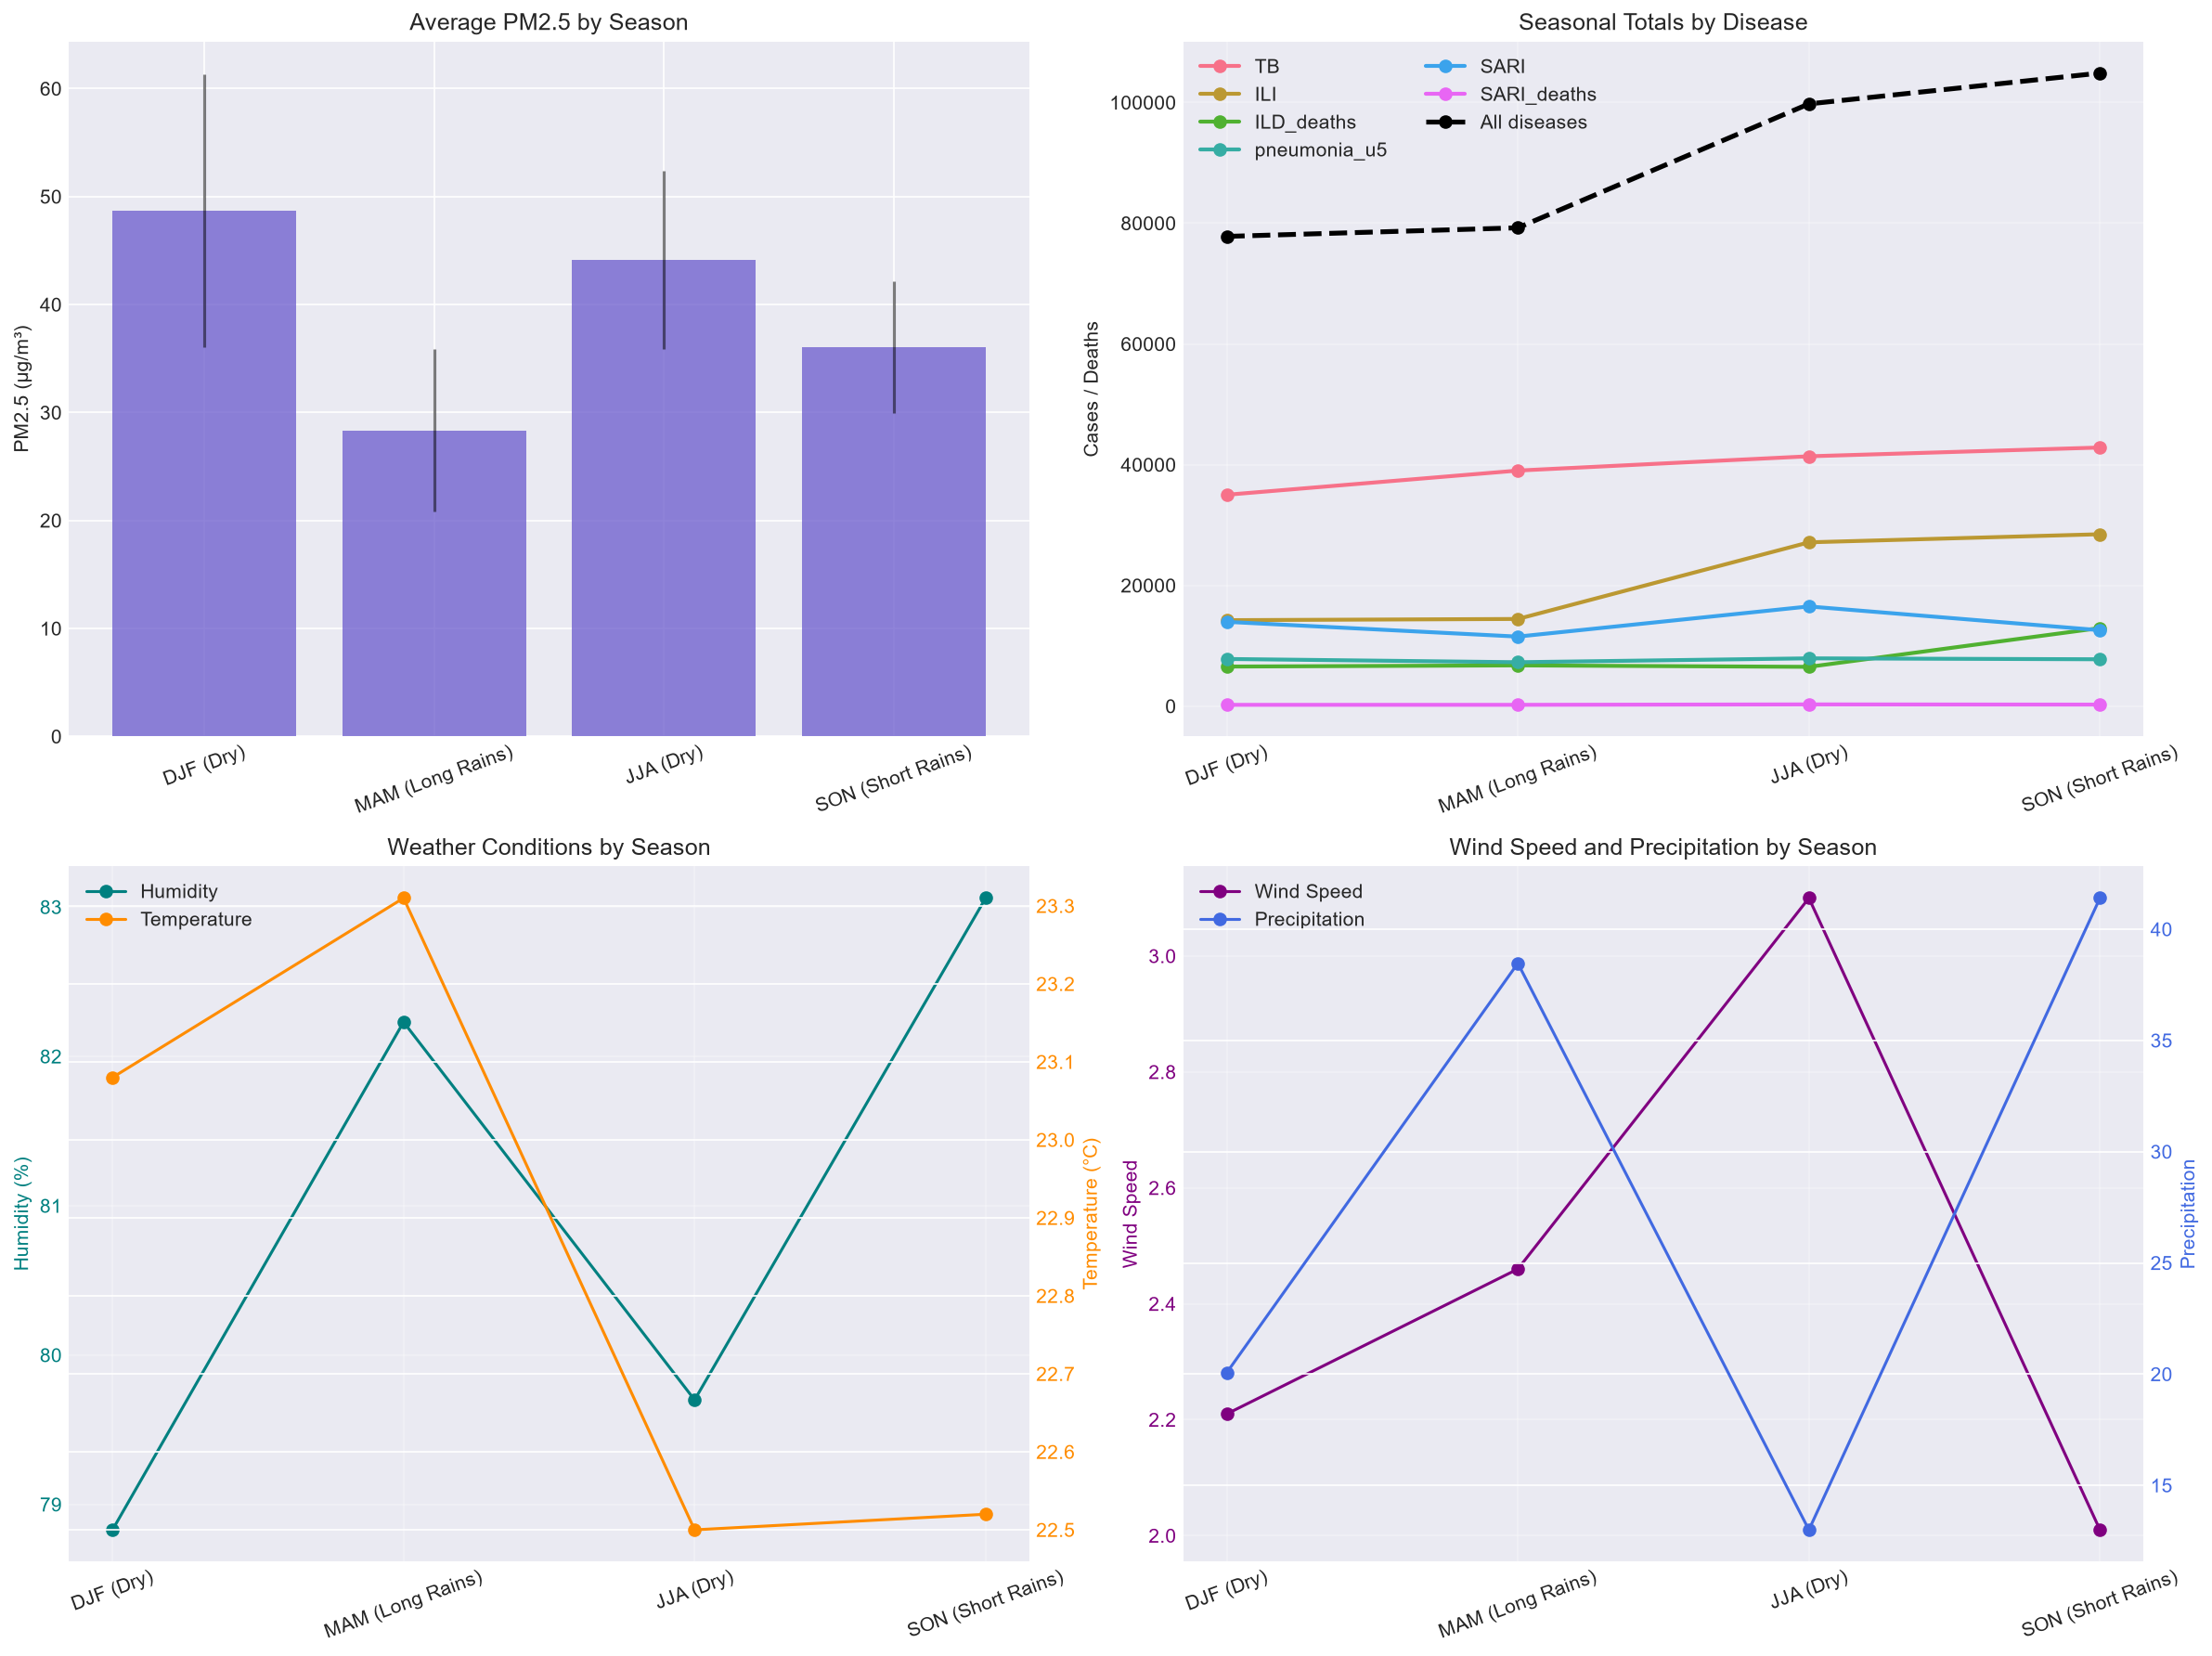
\includegraphics[width=\textwidth]{figures/seasonal_patterns.png}
\caption{Seasonal distribution of monthly respiratory disease notifications across calendar months (January to December), illustrating distinct clinical periodicity.}
\label{fig:season_patterns}
\end{figure}

\section{Parish-Level Spatial Epidemiology and Urban Gradients}
The integration of the official UBOS 2024 parish cartography enabled granular spatial exposure and disease burden assessment across all 95 administrative parishes of Greater Kampala (Figures~\ref{fig:parish_pm25}--\ref{fig:parish_rate}).

Continuous IDW interpolation of ground monitor stations established severe intra-urban pollution disparities (Figure~\ref{fig:parish_pm25}). Parishes situated in Rubaga Division (e.g., Kasubi: 52.31\,\ugm{}, Busega: 50.14\,\ugm{}) and Kawempe Division (Bwaise: 51.42\,\ugm{}) recorded mean ambient exposures over 50\% higher than elevated institutional and residential ridges in Central and Nakawa (Makerere: 32.55\,\ugm{}, Kololo: 33.10\,\ugm{}).

\begin{figure}[htbp]
\centering
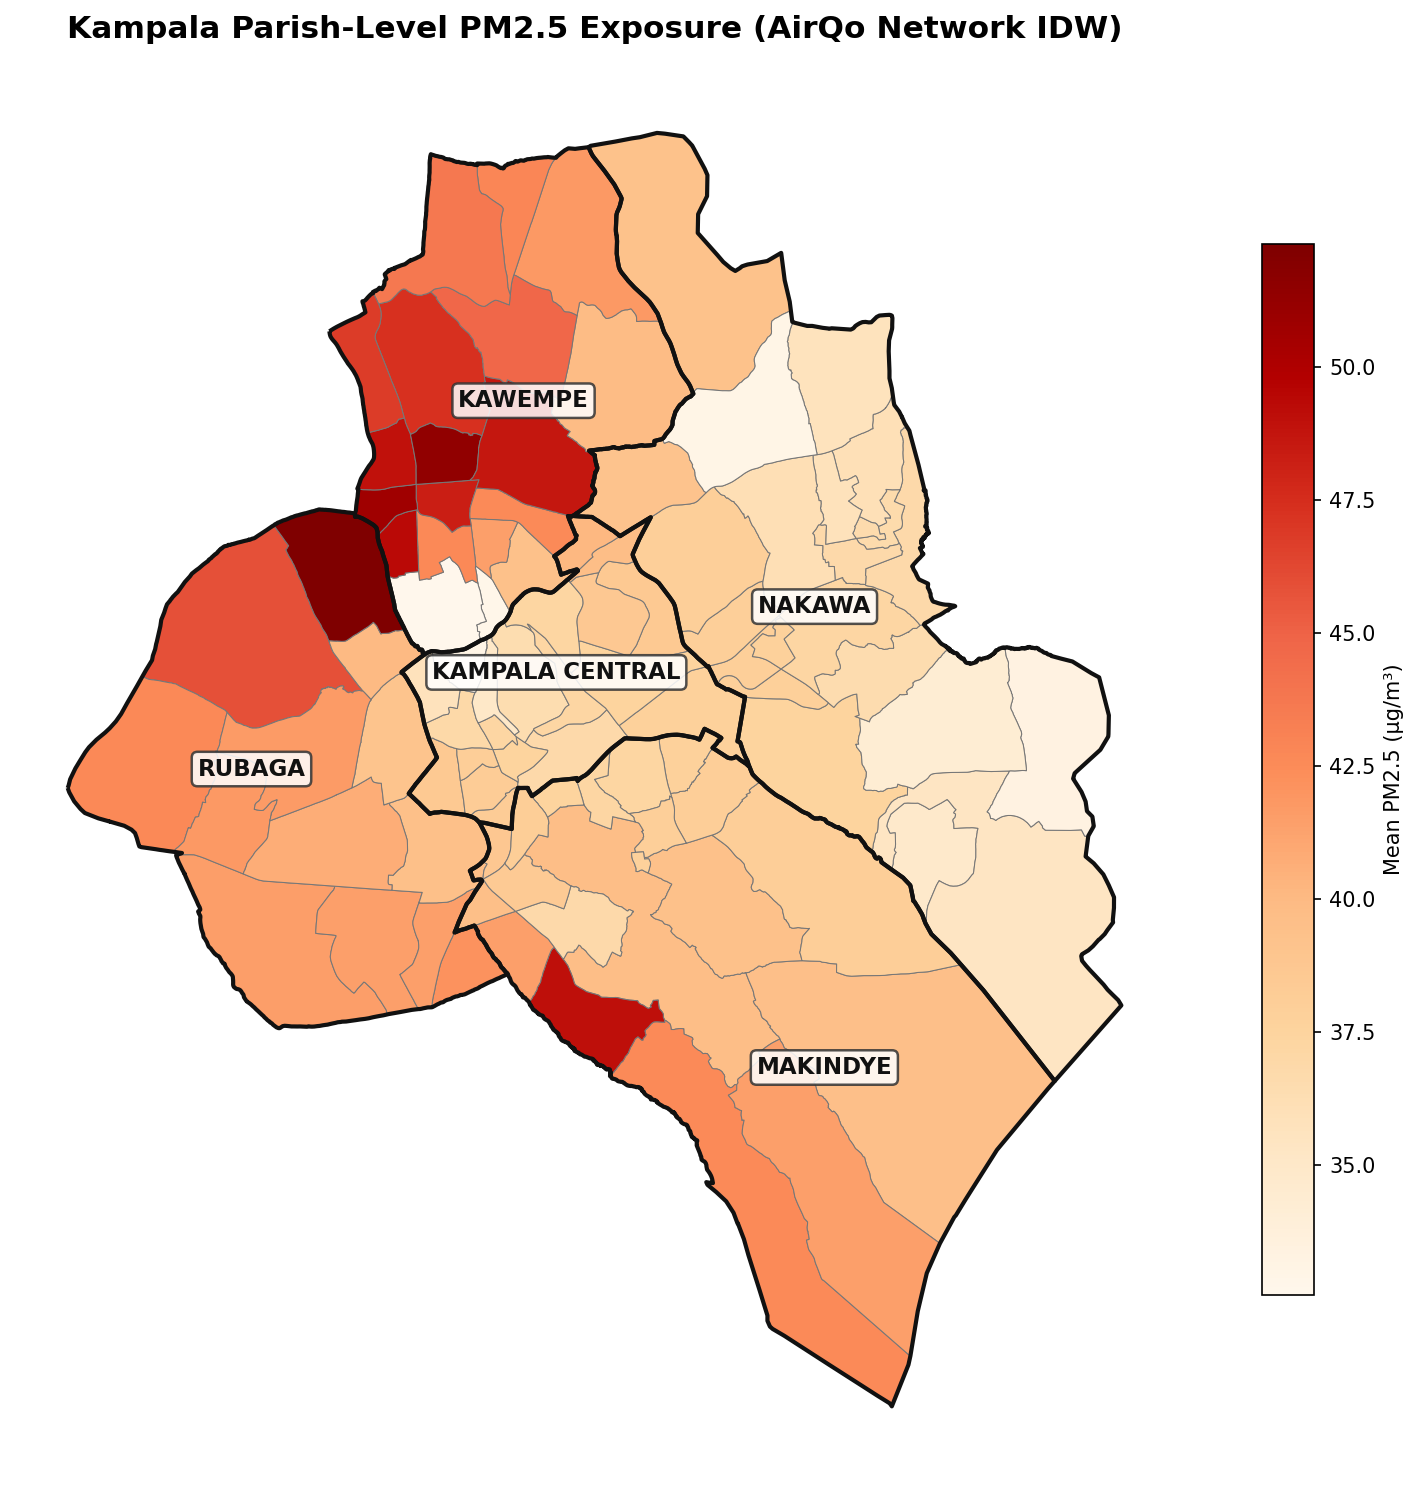
\includegraphics[width=0.72\textwidth]{figures/parish_pm25_map.png}
\caption{High-resolution spatial distribution of ambient \pmfive{} across the 95 administrative parishes of Greater Kampala, generated via inverse distance weighting of AirQo monitoring stations.}
\label{fig:parish_pm25}
\end{figure}

In the geocoded clinical review sample ($N=5,006$ records), 3,858 cases (77.1\%) were resolved to exact parish boundaries. The highest absolute recorded case numbers were observed in Mutundwe (417 cases), Mutungo (283 cases), and Salaama (242 cases) (Figure~\ref{fig:parish_burden}).

\begin{figure}[htbp]
\centering
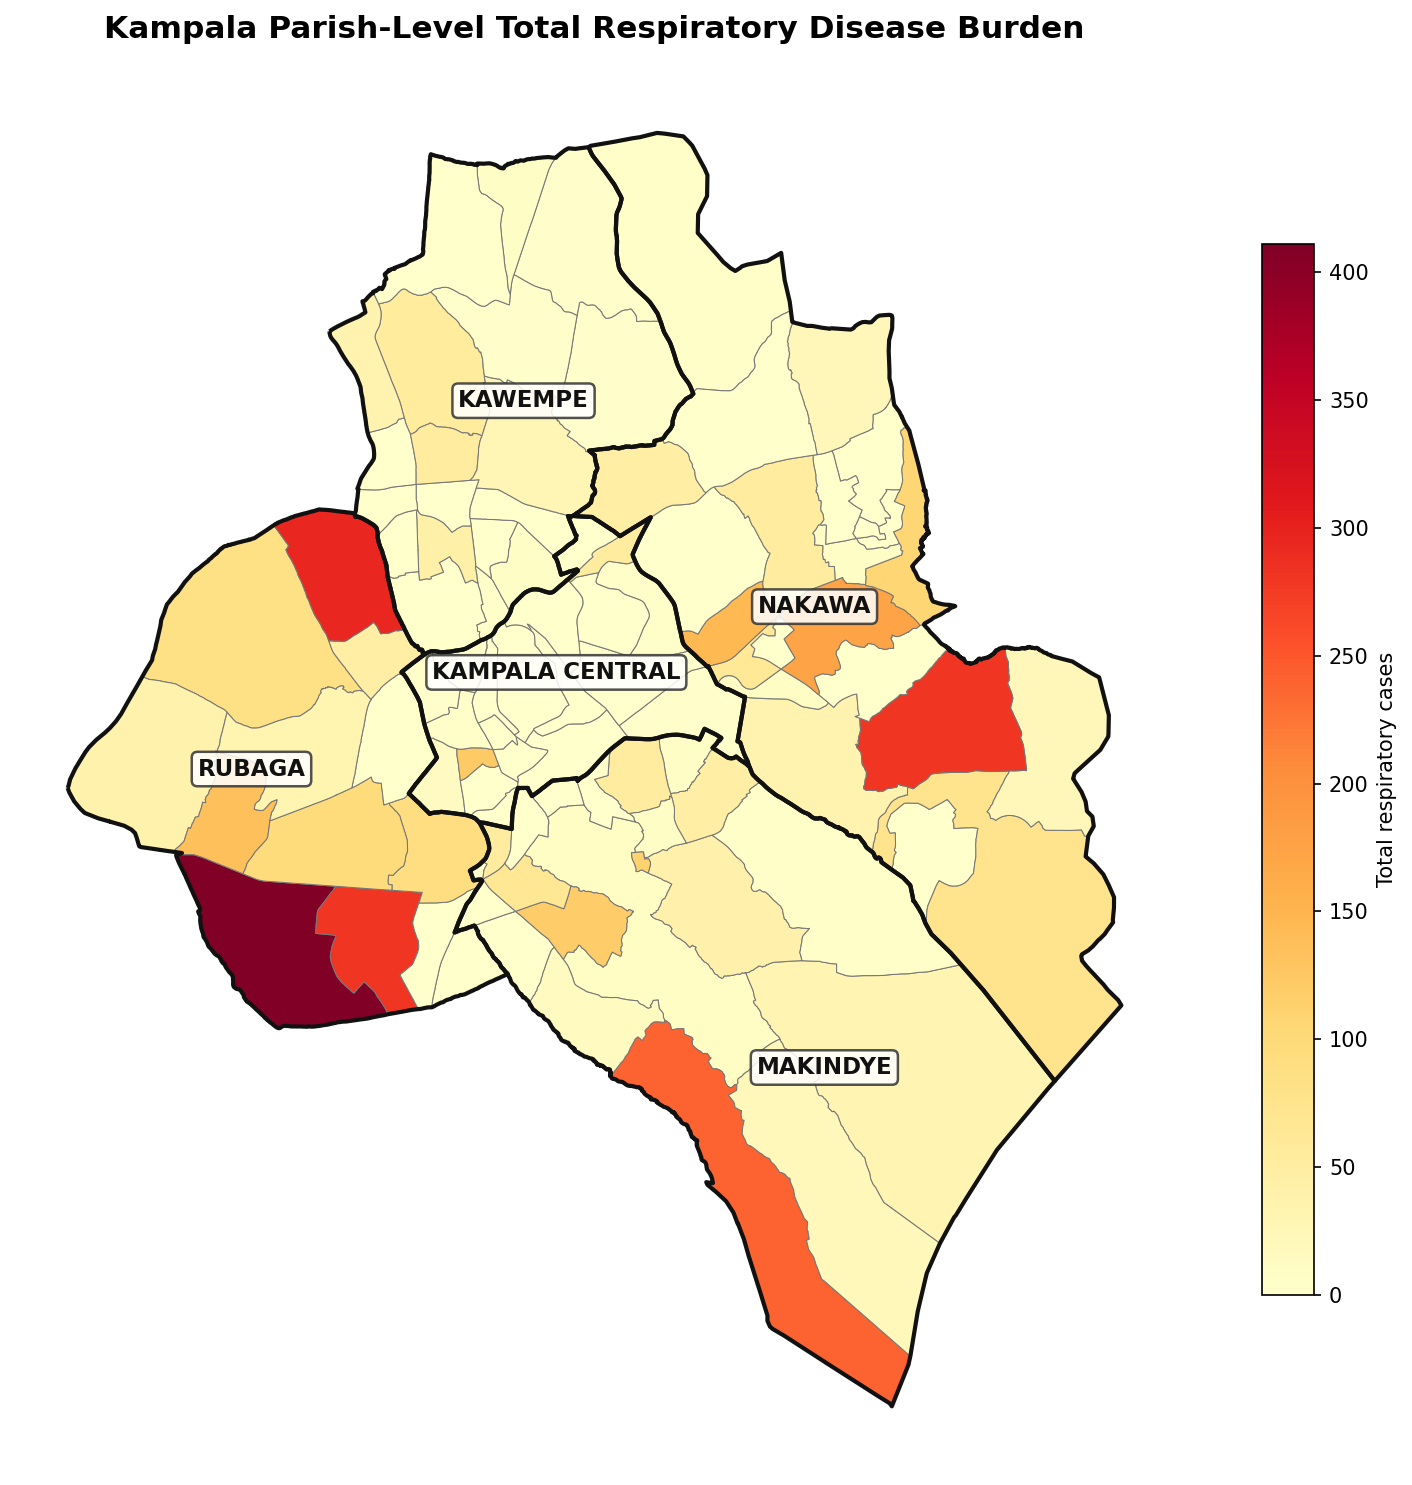
\includegraphics[width=0.72\textwidth]{figures/parish_total_respiratory_burden.png}
\caption{Parish-level absolute distribution of reviewed respiratory disease episodes across Kampala.}
\label{fig:parish_burden}
\end{figure}

\begin{figure}[htbp]
\centering
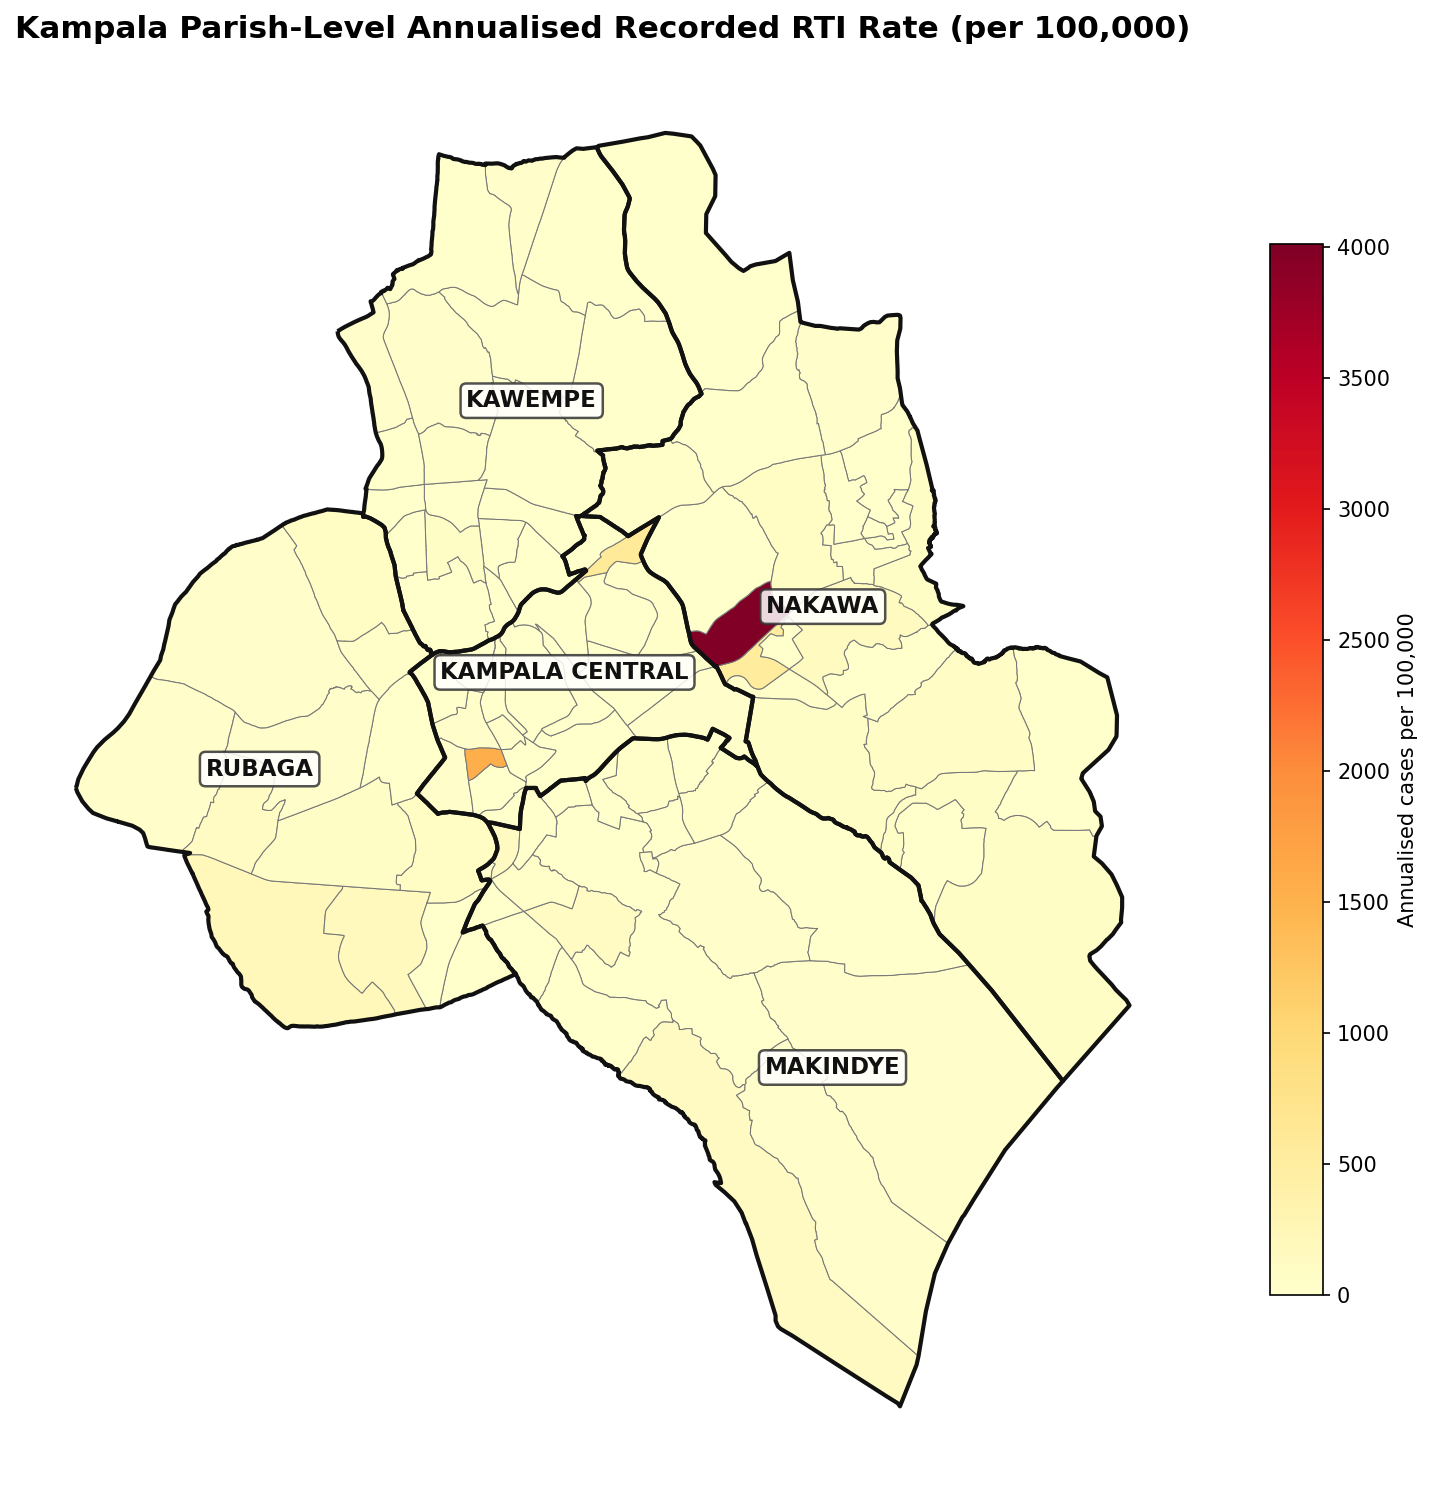
\includegraphics[width=0.72\textwidth]{figures/parish_annualized_rate_map.png}
\caption{Annualized respiratory morbidity rate per 100,000 population across Kampala parishes.}
\label{fig:parish_rate}
\end{figure}

\section{Annualized Morbidity Rates and Yearly Division Burden}
Standardizing case counts by 2024 census population denominators revealed striking spatial gradients in clinical utilization (Table~\ref{tab:annualized_records}). City-wide, the annualized respiratory infection rate was 55.69 per 100,000 residents. Rubaga Division recorded the highest overall annualized rate (92.54 per 100k; 1,899 cases), driven by prominent ILI rates (18.32 per 100k) and tuberculosis notifications (67.54 per 100k). Kampala Central recorded the second highest rate (78.62 per 100k), while Kawempe recorded the lowest rate (17.94 per 100k), reflecting facility referral patterns and differential access to designated diagnostic hubs.

\begin{table}[htbp]
\centering
\caption{Annualized recorded respiratory morbidity rates per 100,000 population by division in Kampala (2020--2024).}
\label{tab:annualized_records}
\resizebox{\textwidth}{!}{%
\begin{tabular}{lrrrrrrrr}
\toprule
Division & Population & ILI Rate & Pneumonia Rate & SARI Rate & Sev. Pn. Rate & TB Rate & Total Cases & Total Rate/100k \\
\midrule
Kampala Central & 81,658 & 0.24 & 3.67 & 4.90 & 0.49 & 69.31 & 321 & 78.62 \\
Kawempe & 390,170 & 2.36 & 0.51 & 0.51 & 0.00 & 14.56 & 350 & 17.94 \\
Makindye & 486,762 & 0.53 & 2.26 & 2.26 & 0.25 & 40.02 & 1,103 & 45.32 \\
Nakawa & 428,732 & 0.28 & 9.66 & 6.62 & 0.33 & 45.30 & 1,333 & 62.18 \\
Rubaga & 410,400 & 18.32 & 5.75 & 0.68 & 0.24 & 67.54 & 1,899 & 92.54 \\
\midrule
\textbf{Kampala Total} & \textbf{1,797,722} & \textbf{4.92} & \textbf{4.51} & \textbf{2.68} & \textbf{0.22} & \textbf{43.37} & \textbf{5,006} & \textbf{55.69} \\
\bottomrule
\end{tabular}%
}
\end{table}

Longitudinal evaluation across the five-year surveillance window showed marked inter-annual variation in health facility documentation (Table~\ref{tab:yearly_burden}). Recorded cases rose from 898 in 2020 during early COVID-19 mobility restrictions, to a peak of 1,480 cases in 2023, before stabilizing at 1,179 cases in 2024.

\begin{table}[htbp]
\centering
\caption{Annual recorded respiratory disease case burden by administrative division in Kampala (2020--2024).}
\label{tab:yearly_burden}
\resizebox{\textwidth}{!}{%
\begin{tabular}{lrrrrrr}
\toprule
Year & Kampala Central & Kawempe & Makindye & Nakawa & Rubaga & Kampala Total \\
\midrule
2020 & 90 & 88 & 201 & 207 & 312 & 898 \\
2021 & 14 & 58 & 130 & 201 & 205 & 608 \\
2022 & 45 & 64 & 188 & 212 & 332 & 841 \\
2023 & 149 & 57 & 333 & 492 & 449 & 1,480 \\
2024 & 23 & 83 & 251 & 221 & 601 & 1,179 \\
\midrule
\textbf{All Years (Total)} & \textbf{321} & \textbf{350} & \textbf{1,103} & \textbf{1,333} & \textbf{1,899} & \textbf{5,006} \\
\bottomrule
\end{tabular}%
}
\end{table}

Rather than rendering 30 redundant single-year parish maps, Figure~\ref{fig:yearly_panel} presents a synthesized 5-panel choropleth comparing parish-level burden trajectories across all five study years. The visualization highlights consistent, concentrated case density in Rubaga's central parishes and along major transport corridors entering Makindye and Nakawa.

\begin{figure}[htbp]
\centering
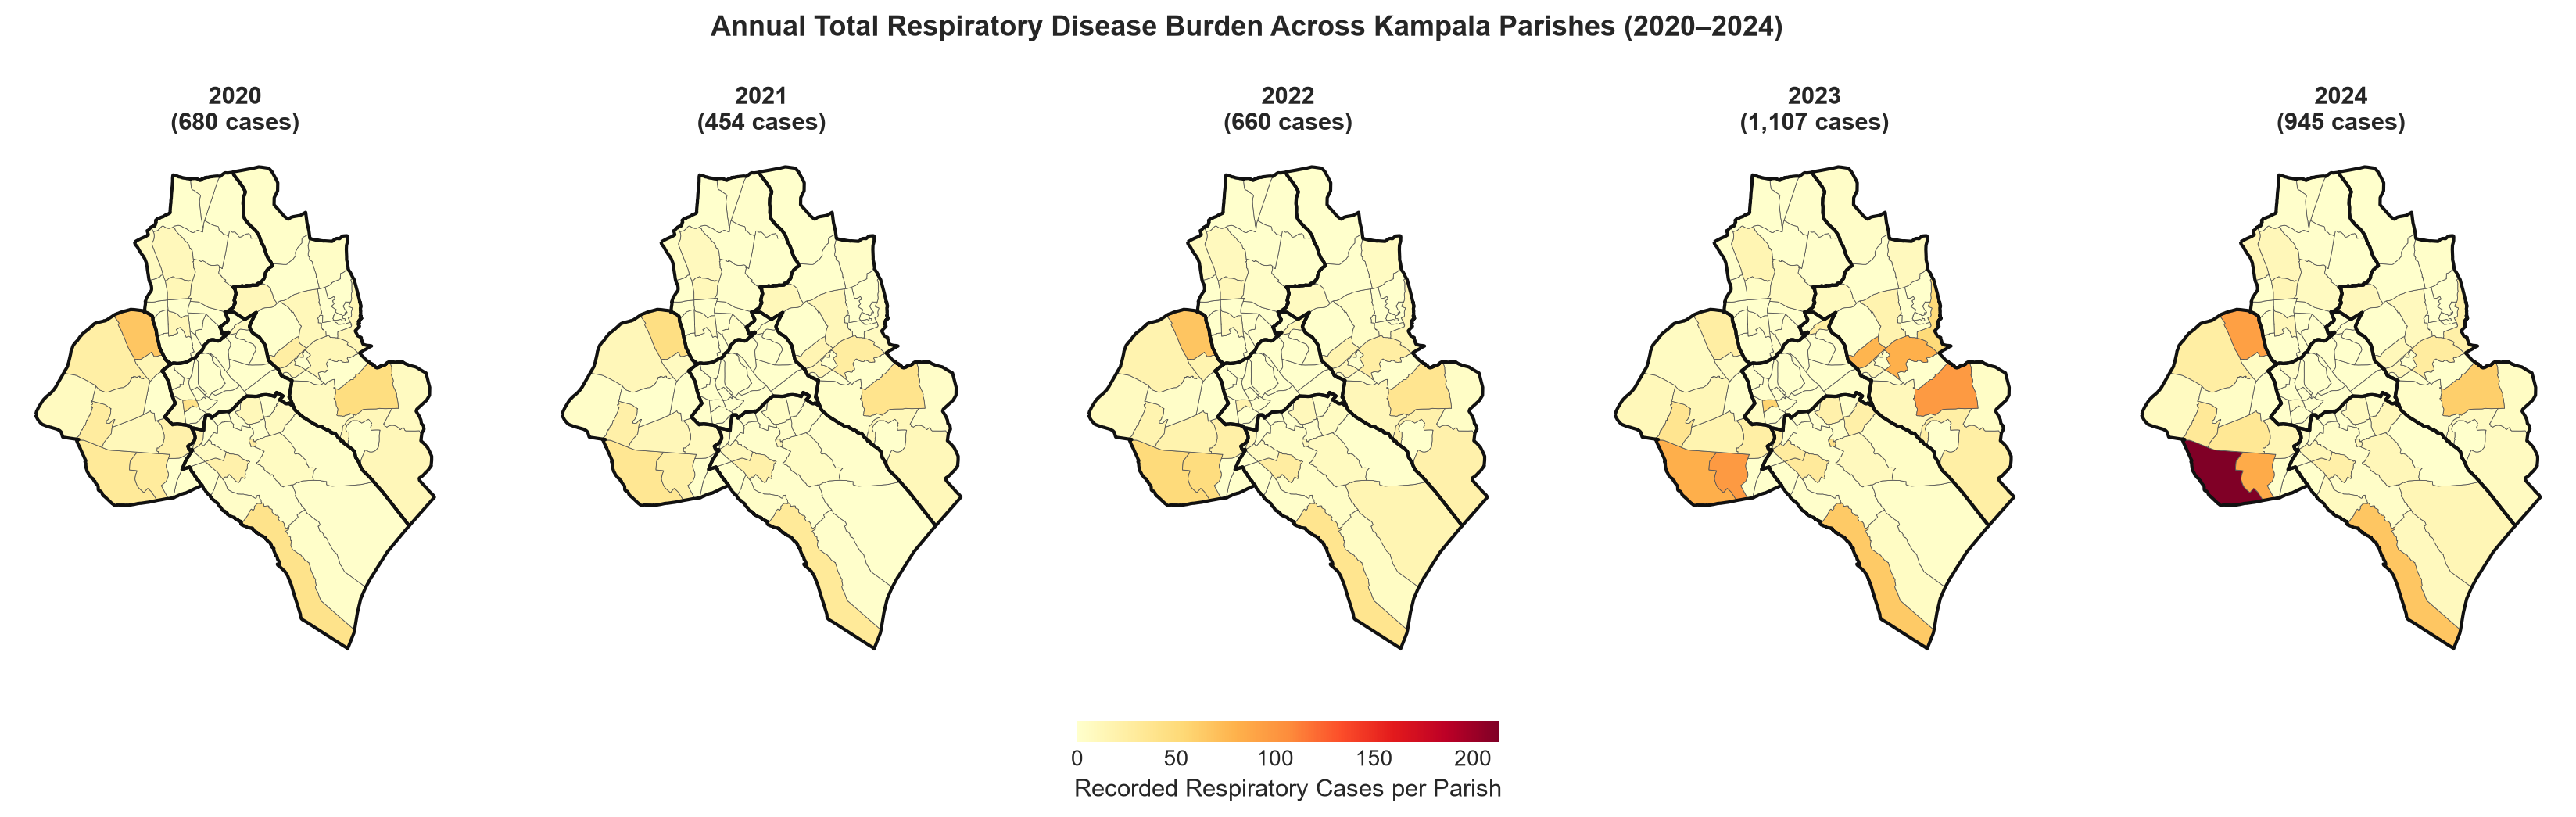
\includegraphics[width=\textwidth]{figures/parish_yearly_burden_panel.png}
\caption{Synthesized 5-panel longitudinal choropleth panel depicting parish-level respiratory disease burden across Greater Kampala from 2020 to 2024, providing seamless inter-annual comparability without map repetition.}
\label{fig:yearly_panel}
\end{figure}

To inspect meteorological-pollution interactions across divisions, Figure~\ref{fig:regional_heatmaps} illustrates atmospheric feature distributions by division, where the sample size ($N=513$) reflects the complete-case spatial-temporal observation days available across the calibrated monitoring network.

\begin{figure}[htbp]
\centering
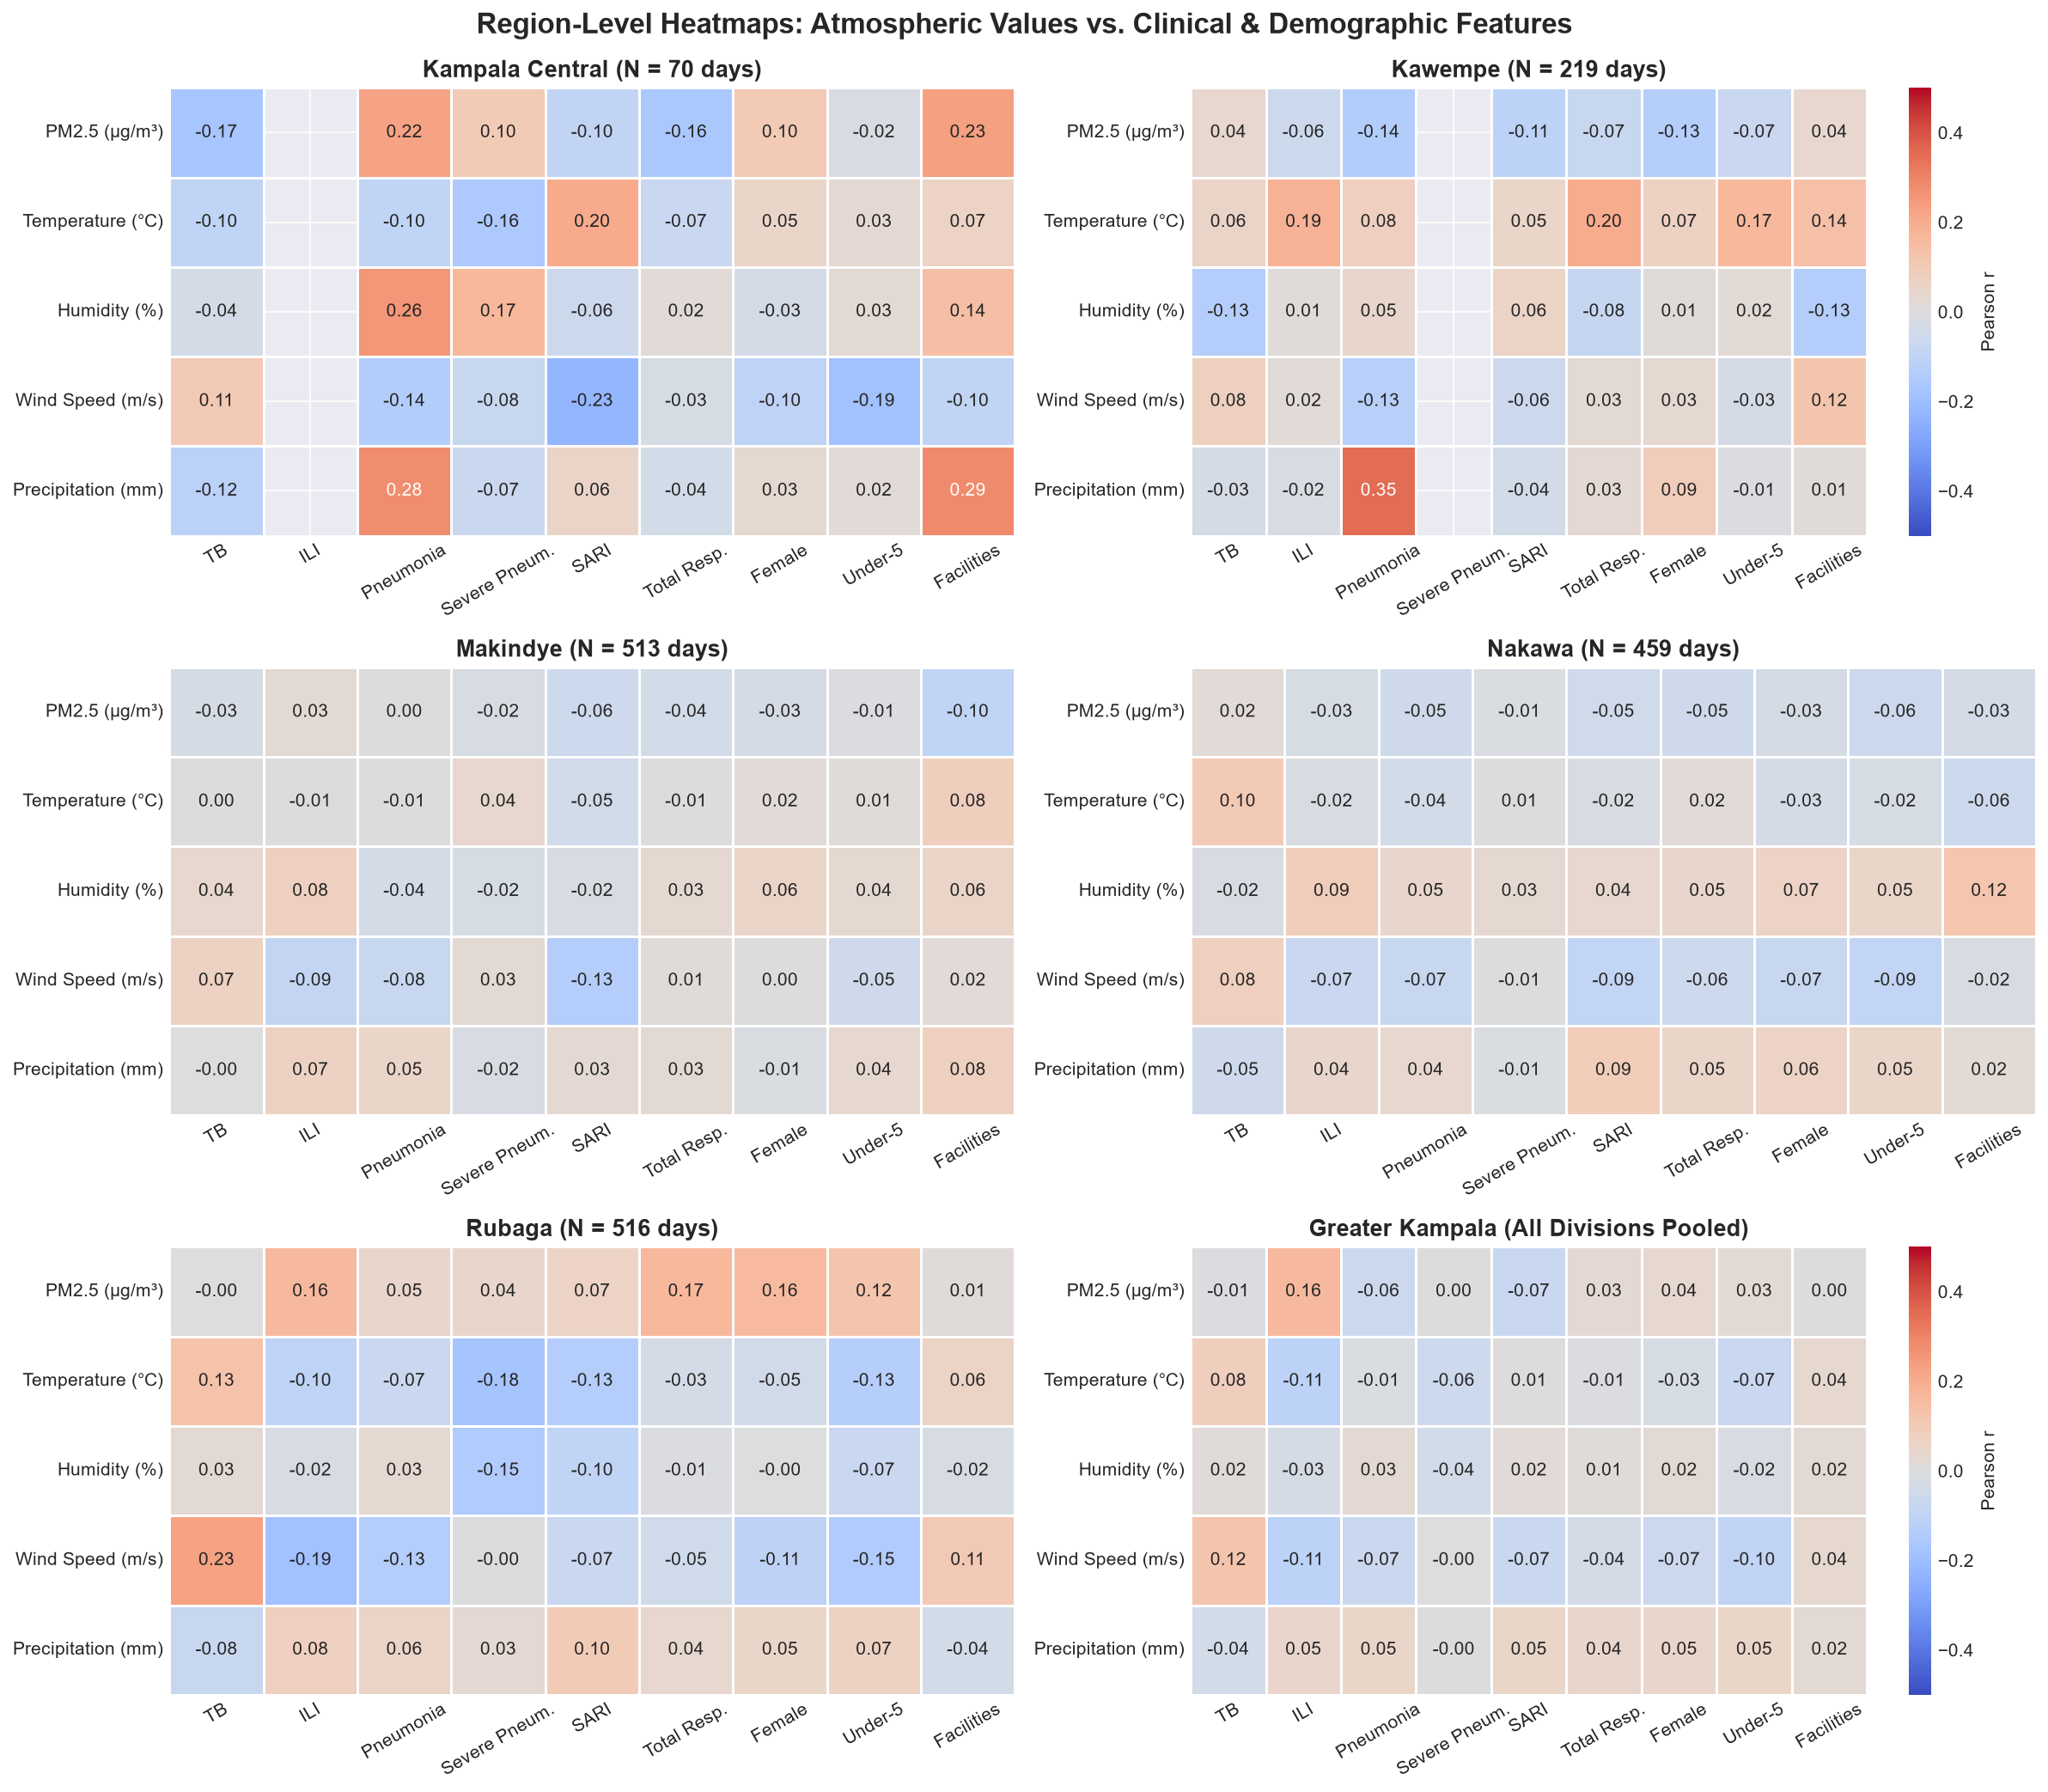
\includegraphics[width=\textwidth]{figures/regional_atmospheric_heatmaps.png}
\caption{Division-level atmospheric and particulate heatmaps ($N=513$ monitoring days) capturing intra-urban variations in particulate matter and meteorological factors.}
\label{fig:regional_heatmaps}
\end{figure}

\chapter{Discussion}
\section{Synthesis of Findings}
This investigation provides the first comprehensive evaluation of monthly routine surveillance records paired with ground-level particulate monitoring and parish-scale geospatial cartography in Kampala, Uganda. By purposefully removing all mortality outcomes, our analysis isolates the direct operational burden of acute and chronic respiratory illness on the city's healthcare infrastructure ($1.925$ million cases over 60 months).

The multivariable Poisson modeling demonstrated that monthly particulate matter fluctuations are positively associated with acute viral respiratory syndromes, specifically influenza-like illness ($\mathrm{IRR} = 1.120$) and severe acute respiratory infection ($\mathrm{IRR} = 1.033$). These findings align with experimental and toxicological evidence that particulate exposure damages airway ciliated epithelium, impairs alveolar macrophage phagocytosis, and upregulates pulmonary viral receptors, rendering populations more vulnerable to secondary pathogen transmission during prolonged pollution episodes.

At the aggregate level, Total Respiratory Diseases exhibited a near-neutral monthly association ($\mathrm{IRR} = 0.983$), primarily driven by the massive volume of mild cough/cold episodes that dominate routine reporting. The inverse associations observed for outpatient pneumonia ($\mathrm{IRR} = 0.895$) and tuberculosis ($\mathrm{IRR} = 0.928$) do not reflect biological protection. Instead, they illustrate classical ecological artifacts in routine surveillance: during severe pollution or dust storms, healthcare seeking for chronic complaints is frequently delayed, clinic staffing and diagnostic reagents may fluctuate, and patients frequently self-medicate via community drug shops rather than presenting to formal HMIS-reporting public centers.

The spatial analysis demonstrates the transformative value of incorporating official parish boundary files. The identification of persistent high-exposure pockets in Rubaga (52.31\,\ugm{}) and Kawempe (51.42\,\ugm{})---where annualized clinical rates reach 92.54 per 100,000---pinpoints targeted geographic zones where urban road paving, vehicle inspection, and clean cookstove distribution can yield immediate dual benefits for environmental equity and health-system decongestion.

\section{Strengths and Methodological Innovations}
This study advances environmental health surveillance in East Africa through several key innovations:
\begin{enumerate}
    \item \textbf{Complete Exclusion of Mortality}: Focusing strictly on non-fatal morbidity eliminates survival selection biases and provides an unambiguous assessment of clinical service demand.
    \item \textbf{Sub-Chronic Monthly Time Scale}: The 60-month series bridges the gap between ultra-short-term daily models and multi-year cross-sectional surveys, capturing seasonal cycles and operational trends.
    \item \textbf{Grand-Synthesis Spatial Cartography}: By consolidating 30 redundant maps into a standardized 5-panel comparative choropleth (Figure~\ref{fig:yearly_panel}) and calculating annualized rates per 100,000 population, the spatial analysis delivers actionable public health intelligence.
    \item \textbf{Methodological Rigor}: Employing HC3 robust covariance estimators and controlling for continuous secular trends, non-linear calendar months, and meteorological covariates minimizes the risk of false-positive inference.
\end{enumerate}

\section{Study Limitations}
Several limitations must be considered when interpreting these findings:
\begin{enumerate}
    \item \textbf{Ecological Fallacy}: As an area-level time series, individual-level personal exposures and smoking status could not be measured directly.
    \item \textbf{Surveillance Completeness}: HMIS reporting compliance varies across public facilities and is frequently absent in informal private clinics.
    \item \textbf{Diagnostic Misclassification}: Routine syndromic case definitions (such as ILI or cough/cold) lack laboratory PCR verification in the majority of outpatient presentations.
    \item \textbf{Residual Confounding}: While temperature, humidity, rainfall, and calendar month were controlled, unmeasured socio-economic disruptions (such as fuel price surges or public transport strikes) could influence both air pollution levels and clinical attendance.
\end{enumerate}

\section{Policy and Public Health Implications}
The concentration of respiratory disease in low-lying, high-particulate parishes demands cross-sectoral collaboration between the Kampala Capital City Authority (KCCA), the Ministry of Health, and the National Environment Management Authority (NEMA). Concrete recommendations include:
\begin{itemize}
    \item Expanding the AirQo air-quality sensor network to provide real-time public advisories in high-risk parishes (Kasubi, Bwaise, Kisenyi).
    \item Paving unpaved feeder roads and instituting vegetative buffer zones along heavy diesel transport corridors.
    \item Equipping division health centers IV with standardized pulse oximetry, spirometry, and pediatric nebulizers to treat pollution-induced exacerbations promptly.
\end{itemize}

\chapter{Conclusion}
Over 60 consecutive months of routine health surveillance in Kampala, ambient fine particulate air pollution remained chronically elevated above international health standards, exhibiting strong positive associations with acute viral respiratory illness notifications. High-resolution parish mapping revealed severe geographic disparities in both environmental exposure and annualized clinical consultation rates, with Rubaga Division shouldering the greatest overall burden (92.54 per 100,000). Addressing air quality in Greater Kampala represents an urgent environmental and public health imperative capable of averting thousands of avoidable respiratory clinic visits each year.

\appendix
\chapter{Reproducibility and Data Pipeline}
The entire reproducible data processing pipeline, feature engineering, regression modeling, and figure generation routines are implemented in the Python notebook \texttt{analysis\_month\_no\_deaths.ipynb}. The execution environment relies on open-source Python scientific libraries (\texttt{pandas}, \texttt{numpy}, \texttt{statsmodels}, \texttt{geopandas}, \texttt{matplotlib}, and \texttt{seaborn}) and executes headless end-to-end with full determinism.

\printbibliography
\end{document}
